
%% CLASS MANUAL FOUND IN http://blog.poormansmath.net/latex-class-for-lecture-notes/ %%
%% CLASS AUTHOR Stefano Maggiolo %%
\documentclass[english,course, draft]{Notes}

\title{ INTRODUCTORY ECONOMICS}
\subject{Economics}
\author{Joao Almeida-Domingues}
\email{2334590D@student.gla.ac.uk}
\speaker{Dr. Constantine Sorokin}
\date{07}{01}{2019}
\dateend{24}{05}{2019}
\place{University of Glasgow}
\usepackage[backend=biber, style=reading]{biblatex}
\bibliography{refEco}
\usepackage{csquotes}
\newcommand\quo[1]{\begin{displayquote}\ita{\large{#1}}\end{displayquote}}

\graphicspath{{assets/}}



 %%%%% GENERAL MATHEMATICAL NOTATION SHORTCUTS %%%%%
 
\newcommand{\n}{\mathbb{N}}
\newcommand{\z}{\mathbb{Z}}
\newcommand{\q}{\mathbb{Q}}
\newcommand{\cx}{\mathbb{C}}
\newcommand{\real}{\mathbb{R}}
\newcommand{\field}{\mathbb{F}}
\newcommand{\ita}[1]{\textit{#1}}
\newcommand{\oneton}{\{1,2,3,...,n\}}
\newcommand\ef{\ita{f} } 
\newcommand\inv[1]{#1^{-1}}
\newcommand\setb[1]{\{#1\}}
\newcommand\en{\ita{n }}
\renewcommand\qedsymbol{QED} %\qedhere to force QED in place
\newcommand{\TODO}[1]{\mymarginpar{TODO: #1}}

%%%%%%%%%%%%%%%%PACKAGES%%%%%%%%%%%%%%%%%%%%%%%%%%%%%
\usepackage{amsmath,amsthm,amssymb} %maths
\usepackage{hyperref,framed,color} %layout
% framed :  \begin{shaded,frame,snugshade or leftbar} \definecolor{shadecolor}{rgb}{XYZ} to change color
%fancybox: \shadowbox,ovalbox or doublebox
%%%%%%%%%%%%%%%%%%%%%%%%%%%

%%%CLASS SHORTCUTS%%%%
%\lecture{day}{month}{year} for margin note
%\begin{theorem} sdfsdf\end{theorem}
%\begin{proposition} dfsdfs\end{proposition}
%\begin{lemma} dsfsd \end{lemma}
%\begin{corollary} f ffew \end{corollary}
%\begin{definition} fwewef w \end{definition}
%\begin{example} feww e\end{example}
%\begin{exercise} wefwe \end{exercise}
%\begin{remark} wef we \end{remark}
%\begin{fact} wefe \end{fact}
%\begin{problem} wef ew \end{problem}
%\begin{conjecture} ewfew \end{conjecture}
%\begin{claim} few w \end{claim}
%\begin{notation} fewf \end{notation}

\begin{document}
\newpage

\section{Microeconomics}

\subsection{Introduction}

\lecture{10}{01}{2019}
We start our journey into the science of economics by establishing its first principles. In particular, we'll focus on:

\begin{itemize}
	\item How individuals make choices?
	\item How individual choices interact?
	\item How those interactions, when combined, give rise to much more complex \ita{economy-wide} interactions
\end{itemize}

\defn{Economy}{A system for coordinating society's productive activities}

\defn{Economics}{The science which studies the production, distribution and consumption of goods}

\par{Most modern day economies are \ita{market economies} \ref{intro:market}, instead of being centrally controlled by an institution \ref{intro:command}, their organisation rely on the many firms and individuals' decisions (in general, people produce and buy whatever they feel like). Adam Smith first observed how this system of individuals making isolated decisions in pursuit of their own interests \ref{intro:hand} could bring about gains to society as a whole in his 1776 \ita{magnum opus - The Wealth of Nation}. In this work he coined the now ubiquitous term of the \ita{invisible hand}.}

\quo{... every individual necessarily labours to render the annual revenue of the society as great as he can. He generally, indeed, neither intends to promote the public interest, nor knows how much he is promoting it. By preferring the support of domestic to that of foreign industry, he intends only his own security; and by directing that industry in such a manner as its produce may be of the greatest value, he intends only his own gain, and he is in this, as in many other cases, led by an invisible hand to promote an end which was no part of his intention.}

\defn{Market Economy}{Decisions about production and consumption are made by individual producers and consumers~\label{intro:market}}

\defn{Command Economy}{The government determines what goods should be produced, how much should be produced and the price at which the goods are offered for sale~\label{intro:command}}

\defn{Invisible Hand}{The way in which the individual pursuit of self-interest can lead to good results for society as a whole~\label{intro:hand}}

\defn{Microeconomics}{The branch of economics that studies how people make decisions and how these interact}



\par{Things don't always go smoothly when the invisible hand is the only guiding force in action. When the individuals' pursuit of self-interest brings about detrimental effects to society, economies experience \ita{market failure~\ref{intro:failure}}. An aggregate of these failures can lead to entire periods of general ill-being~\ref{intro:rec}. These fluctuations between periods of greater~\ref{intro:growth} and lesser wealth are , however,  a common feature of modern economies which macroeconomists occupy themselves with~\ref{intro:macro}}

\defn{Macroeconomics}{The branch of economics that studies the overall ups and downs in the economy as a whole~\label{intro:macro}}

\defn{Market Failure}{When the individual pursuit of self-interest leads to bad results for society as a whole~\label{intro:failure}}

\defn{Recession}{A downturn in the economy~\label{intro:rec}}

\defn{Economic Growth}{The growing ability of the economy to produce goods and services~\label{intro:growth}}

\subsection{Underlying Principles of Individual Choice}

\begin{enumerate}
	
	\item{Scarce resources mandate choices}
	\item{The true cost of an item is its opportunity cost~\ref{principles:cost}}
	\item{"How Much" decisions, require making \ita{trade-offs}~\ref{principles:trade-off} at the margin~\ref{principles:margin}}
		\rem{Not all decisions are binary, some involve assessing the costs and benefits at different stages (e.g. dropping out of college in your last semester vs first)}
	\item{People usually respond to incentives~\ref{principles:incentive}, exploiting opportunities to make themselves better off~\label{principles:incentiveP}}
		\rem{the principle that people will exploit opportunities to make themselves better off is the basis of all predictions by economists about individual behaviour}
	

	\defn{Opportunity Cost}{What you must give up in order to get something else~\label{principles:cost}}
	\defn{Trade-Off}{Comparing the costs and benefits of a choice~\label{principles:trade-off}}
	\defn{Marginal Decisions}{Decisions that occur at the cost-benefit margin~\label{principles:margin}}
	\defn{Marginal Analysis}{The study of marginal decisions}
	\defn{Incentive}{Anything which rewards behaviour changes~\label{principles:incentive}}
	
\subsection{Principles of the Interaction of Individual Choices}



	\item{Specialisation brings about gains from trade}
	\item{Markets move towards equilibrium~\ref{principles:equilibrium}}
		\rem{This follows from \ref{principles:incentiveP}}
	\item{Resources should be used efficiently to achieve society's goals}
		\rem{Occasionally there are overriding reasons to efficiency, like equity~\ref{principles:equity}}
	\item{Markets tend towards efficiency}
	\item{When markets don't achieve efficiency, government intervention can improve society's welfare}
	
\subsection{Principles of Economy-Wide Interactions}

	\item{One person's spending is another's income}
		\rem{In a recession, for example, this causes a synergic effect. People lose jobs, they have less money, they spend less, other people have less, they also lose their jobs etc.}
	\item{Overall Spending Sometimes Gets Out of Line with the Economy's Productive Capacity}
		\rem{Underspending often leads to recessions. Overspending leads to \ita{inflation}~\ref{principles:inflation}}
	\item{Government Policies Can Change Spending}
	
\end{enumerate}
	
	\defn{Equilibrium}{A situation in which individuals cannot make themselves better off by doing something different~\label{principles:equilibrium}}
	\defn{Efficient Economy}{Resources are used efficiently when they are used in a way that has fully exploited all opportunities to make everyone better off}
	\defn{Equity}{Allowing for everyone to have his/her fair share~\label{principles:equity}}
	\defn{Inflation}{A rise in prices throughout the economy. This occurs when the amount that people want to buy outstrips the supply, producers can raise their prices and still find willing customers.~\label{principles:inflation}}
	
\section{Economic Models}
\lecture{11}{01}{2019}

In this section:
\begin{enumerate}
	\item Explain the crucial role that models play in economics
	\item Introduce 2 simple models: comparative advantage ; possibility frontier
	\item Explain the difference between normative and positive economics
\end{enumerate}

\subsection{Production Possibility Frontier}
\defn{Model}{ Simplified representation of reality that is used to better understand real-life situations}
	\rem{Models are essential to economics, because their relative simplicity allow economists to hold everything else constant and study how one change affects the overall economic outcome}
	
\defn{Production Possibility Frontier Model}{A curve depicting all maximum output possibilities for two goods, given a set of inputs consisting of resources and other factors. The PPF assumes that all inputs are used efficiently}

\par{The PPF model helps companies evaluate their \ita{production efficiency}. When a company its producing at its \ita{production possibility frontier~\ref{model:ppf}} we say that it is \ita{efficient in production~\ref{model:efProd}}. This however is not enough to classify an economy as efficient. After the goods are produced it is necessary to produce the mix of goods that people want to consume, if this is the case we talk of \ita{efficient in allocation~\ref{model:efAl}}}

\defn{PPF}{The limit at which an economy as maximised the usage of resources, maximising its production capacity~\label{model:ppf}}
\defn{Efficient in Production}{When an economy is in its production possibility frontier; we say that the economy is efficient in production~\label{model:efProd}}
\defn{Efficient in Allocation}{When an economy allocate its resources so that consumers are as well off as possible~\label{model:efAl}}

\begin{figure}[ht]
\centering
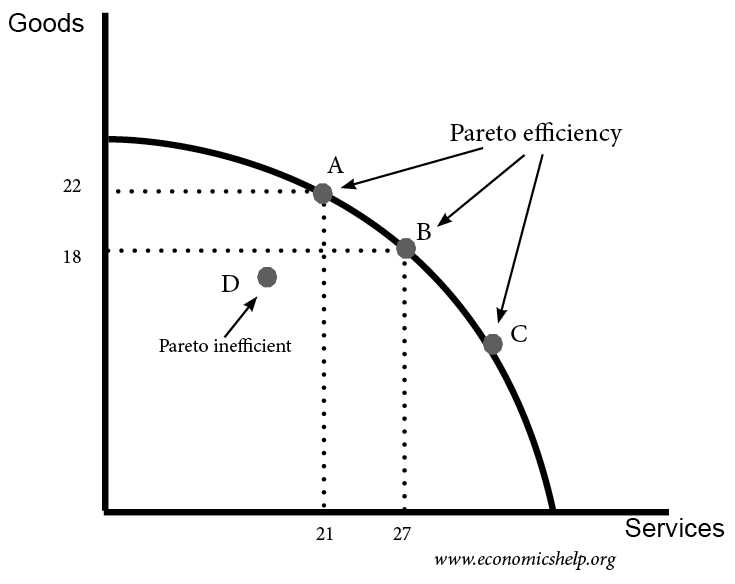
\includegraphics[width=0.8\textwidth]{ppf.png}
\end{figure}

\par{We can estimate the \ita{opportunity cost} of producing different goods by looking at the gradient of the line between the current point and the point we wish to investigate. The steeper the gradient (for greater $\Big|\frac{\mathrm{d}y}{\mathrm{d}x}\Big| $), the higher the opportunity cost}

\par{We can also look at the \ita{economic growth}. Economic growth means an expansion of the economy's production possibilities. Hence we should expect the graph to be scaled in all directions. This can come about due to an increase in the \ita{factors of production~\ref{model:prod}} (e.g. new hangar, whereby a company can produce more aircrafts of type A without reducing the number of type Bs). Or by advances in \ita{technology}(e.g. semicondutors industry, transistors, home pc)}

\defn{Factors of Production}{Any resource needed for the creation of a good or service (land, labor, capital and entrepreneurship)~\label{model:prod}}


\subsection{Comparative Advantage}

\par{The basic idea behind this model is that \ita{it makes sense to produce that which you're particularly good at producing, and buy that which you are not}. By choosing to produce the product (A) which as a lower opportunity-cost, the factors of production are freed from the other possible products. Hence this others can be obtained from trading with another entity which also benefits, since the product being traded has a higher opportunity-cost for them.~\ref{advantage}}

\defn{Comparative Advantage~\label{advantage}}{When an entity's opportunity-cost for some product is lower than that of some other entity's}

\begin{figure}[ht]
\centering
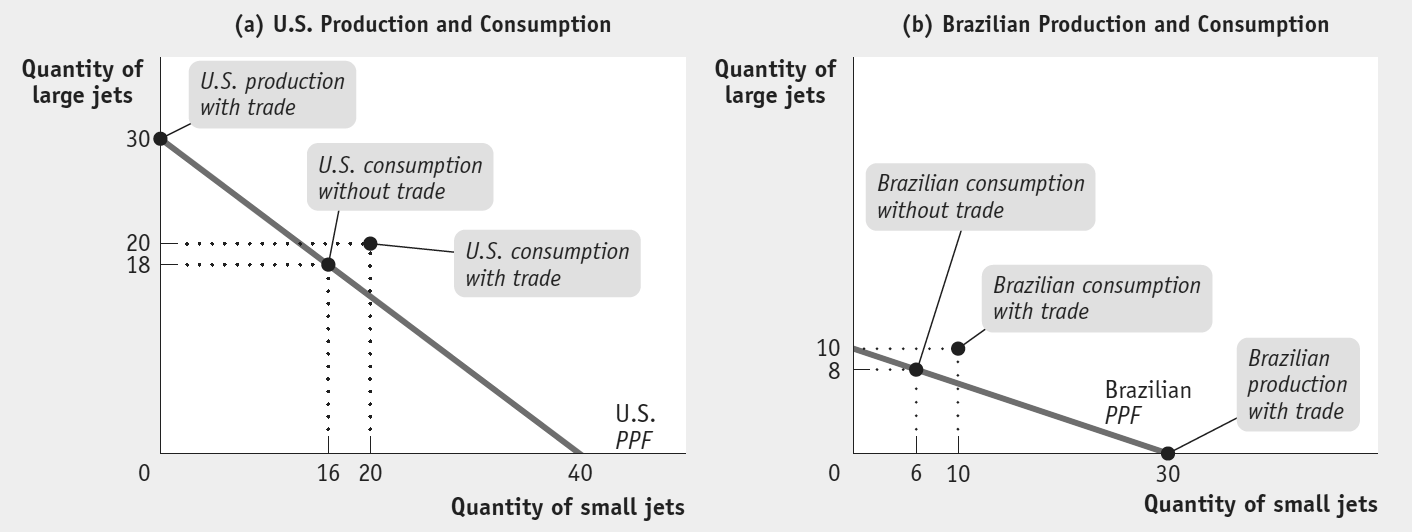
\includegraphics[width=0.9\textwidth]{jetsTrade.png}
\end{figure}

\rem{Note, how by trading, both production and consumption increase for both countries}

\defn{Absolute Advantage}{when an entity can produce more output per worker than other countries}

\par{Note that this doesn't mean that trading is no longer beneficial, what matters is the \ita{net gain}.It
does not matter whether it takes Brazil more resources than the United States to make a small jet; what matters for trade is that for Brazil the opportunity cost of a small jet is lower than the U.S. opportunity cost. So Brazil, despite its absolute
disadvantage, even in small jets, has a comparative advantage in the manufacture of small jets}

\begin{figure}[ht]
\centering
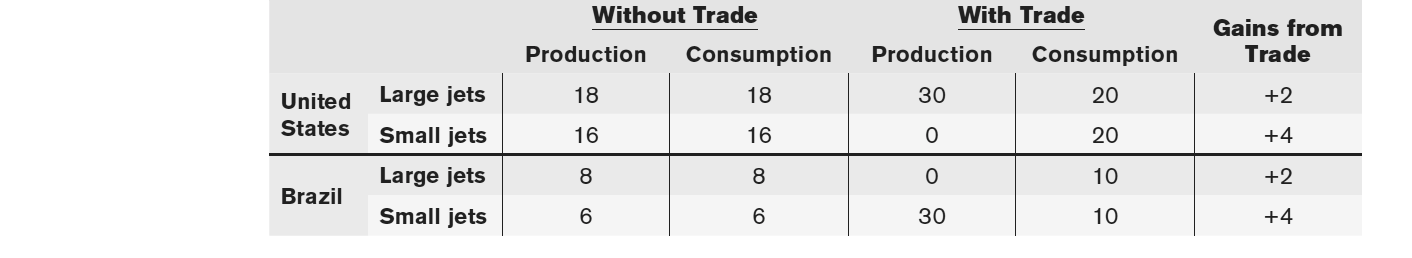
\includegraphics[width=0.9\textwidth]{jetsTrade2}
\end{figure}

\subsection{Interpreting the Simplification of Models}
\lecture{15}{01}{2019}
\par{The models used as examples above are grossly oversimplified, this of course has negative consequences, in particular makes the conclusions derived from them less reliable. Yet, as previously stated they are useful because they  illustrate best the fundamentals of economics.}

\par{The \ita{circular-flow diagram} for example, allow us to analyse the complex transactions that take place in an economy by looking at \ita{the flow of things}, and \ita{the flow of money}. The simplest of these has only 2 entities  \ref{flow:house} \ita{households} and \ref{flow:firms} \ita{firms}, whose interaction is mediated by two types of markets those for \ref{flow:goods} \ita{goods and services} and those for the \ref{flow:factor} \ita{factors of production}.}

\defn{Household~\label{flow:house}}{A person or group of people who share their income}
\defn{Firms~\label{flow:firms}}{An entity which produces goods and services}
\defn{Goods \& Services Market~\label{flow:goods}}{Where firms sell their products to households}
\defn{Factor Market~\label{flow:factor}}{Where firms buy the factors of production (e.g. job market)}
\newpage

\begin{figure}[ht]
\centering
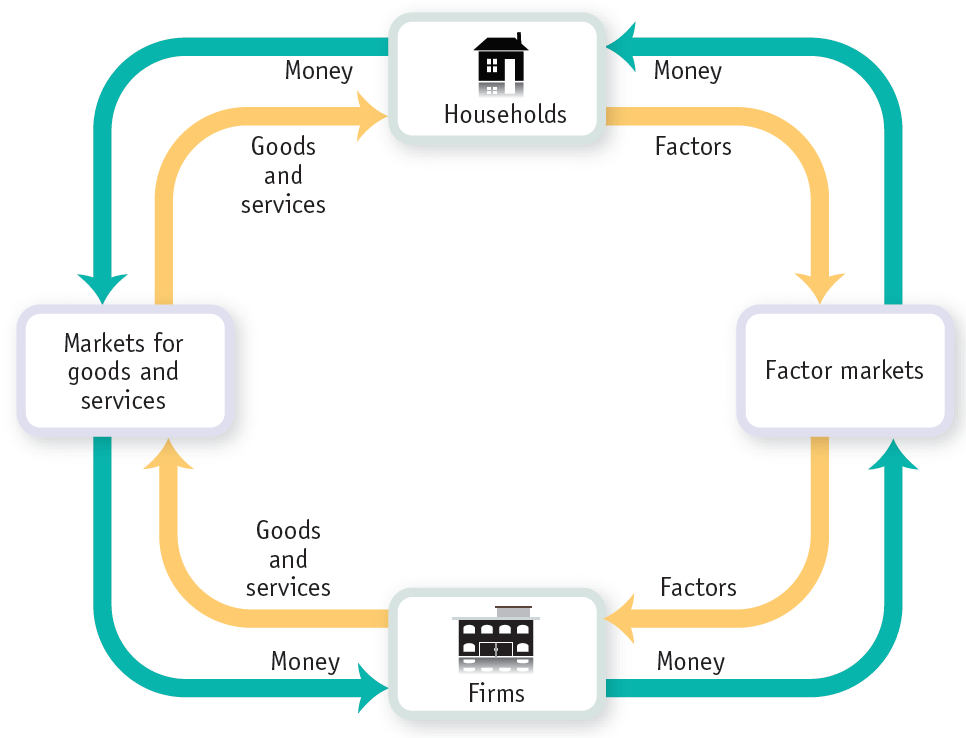
\includegraphics[width=0.7\textwidth]{flow.png}
\end{figure}

\rem{Note how the flows are opposite to each other, since \ita{in general} when an entity puts x into a system it gets y. As an illustration consider how the flow of money \ita{into} the market of goods \textbf{from} the household, leads to a flow of goods \ita{from} the market \textbf{into} the household.}

\par{We need to once again bear in mind the shortcomings of this model, for example the distinction between households and firms is not always clearly distinct, firms interact with each other and the government is not illustrated}

\subsection{Economic Analysis: Positive vs Normative}

\defn{Positive Economics}{Concerns itself with establishing matters of fact. It is therefore purely descriptive, it is able to provide right and wrong answers, but it does not pass any value judgments}

\defn{Normative Economics}{Prescriptive. It involves recommending courses of action to take in order to optimise an economy}

\rem{Note that even though positive economics deals with facts, and does not aim to prescribe behaviour, its conclusions can still be used to guide policy (e.g. politicians might enact certain policies based on forecasts)}

\rem{Even though there is no "right" answer \ita{per se} when it comes to normative economics, the reason it can still be used to guide public policy is because economists are able to agree on a certain course of action, regardless of their own personal values. Just like in ethics for example, where most scholars do not agree that there is one and one only way to live the \ita{good life} , yet most (if not all) agree that to kill an innocent child is morally blameworthy. In the realm of economics, think of two policies A and B  which achieve the same purpose, if A's net gains are higher then A is the right/preferable option. (e.g. rent control \& rent subsidies in the US)}

\newpage
\section{Supply and Demand}
\lecture{17}{01}{2019}
\subsection{Model of a Competitive Market}

\defn{Competitive Market}{A market where there exists many buyers and sellers, therefore none of them have the power to influence market prices}

\rem{Not all markets are competitive, if there are only a few major players, then they are able to set market prices}

\par{There are five key elements to the CM model}


\subsection{The Demand Curve}
	
	\par{The price of a product or service, affects the amount of that product that people will want to consume. In general, lower prices lead to higher demand~\ref{demand:law}. One can estimate the demand of a certain product by drawing out a table where we map the amount consumers would \ita{want} to buy for each price~\ref{demand:sch}. We can then observe how much would people be willing to pay for a certain quantity~\ref{demand:quantity}, it is by translating this information into a graph that we get the demand curve~\ref{demand:curve}}
	
	\defn{Law of Demand~\label{demand:law}}{A higher price for a good or service, \ita{other things equal}, leads people to demand a smaller quantity of that good or service}
	
	\defn{Demand Schedule~\label{demand:sch}}{How much of a good or service consumers will want to buy at different prices.}
	
	\defn{Quantity Demanded~\label{demand:quantity}}{actual amount of a good or service consumers are willing to buy at some specific price}
	
	\defn{Demand Curve~\label{demand:curve}}{a graphical representation of the demand schedule. It shows the relationship between quantity demanded and price}
	
	\rem{\textbf{N.B} It is paramount not to confuse quantity demanded with demand. Quantity demanded are the individual points on the demand curve}

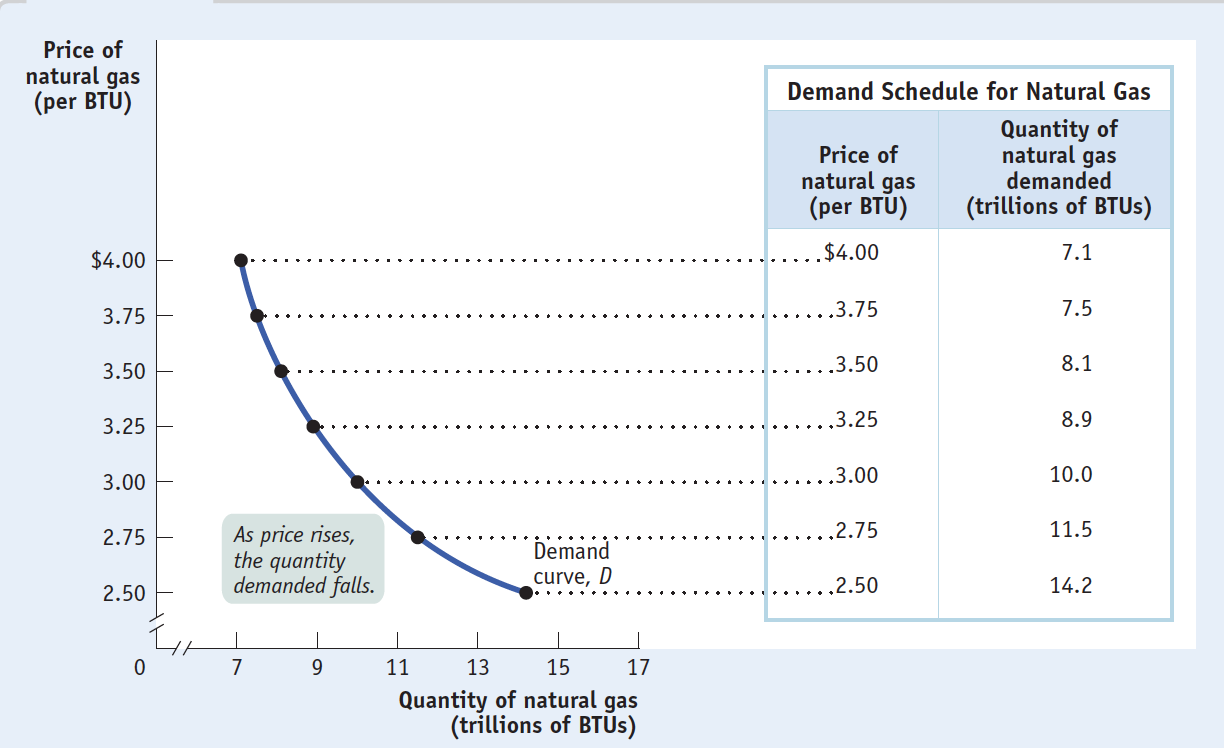
\includegraphics[width=15em]{demandCurve}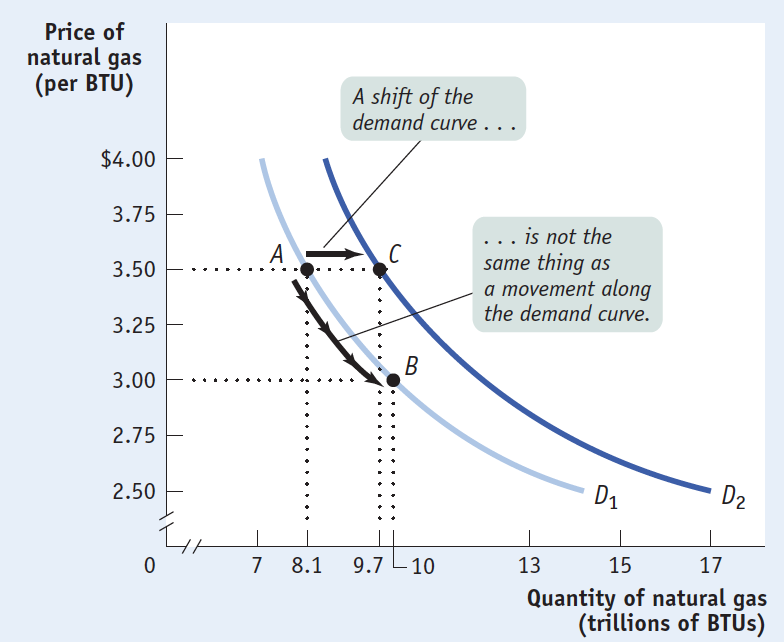
\includegraphics[width=15em]{demandShift}



		
	\par{One important distinction exemplified in the examples above is the graphical representation of a change in the market. We say that there is a shift in demand if \ita{for the same price, the quantity demanded increases}, hence this will translate into a horizontal translation of the curve. A shift of the quantity demanded simply moves us \ita{along the curve} (say for example if there's a sale). There are five major \textbf{non-price determinants} that can lead to a shift in demand:\mymarginpar{see 77 Table 3-1}}
	\begin{enumerate}
	\item  prices of related goods or services. 
	
	\defn{Substitute}{Two goods whose demand and price relation is proportional (price rise of coal leads to demand rise of solar panels)}
	\defn{Complement}{Two goods whose demand and price relation is inversely proportional (increased price of coffee decreased cookie consumption)}
	
	\item income
	
	\defn{Normal Good}{goods whose demand increases, when income increases (holidays)}
	\defn{Inferior Good}{goods whose demand decreases, when income decreases (bus tickets)}
	
	
	\item tastes
	\item expectations
	
	\item number of consumers
	
	\defn{Individual Demand Curve}{illustrates the relationship between quantity demanded and price for an individual consumer.} 
	
	\par{The market demand curve is obtained by performing the horizontal sum of the total number of consumers. If the number of consumers grow and the price remains unchanged, then an increase in demand is necessary.}
		\begin{figure}[ht]
\centering
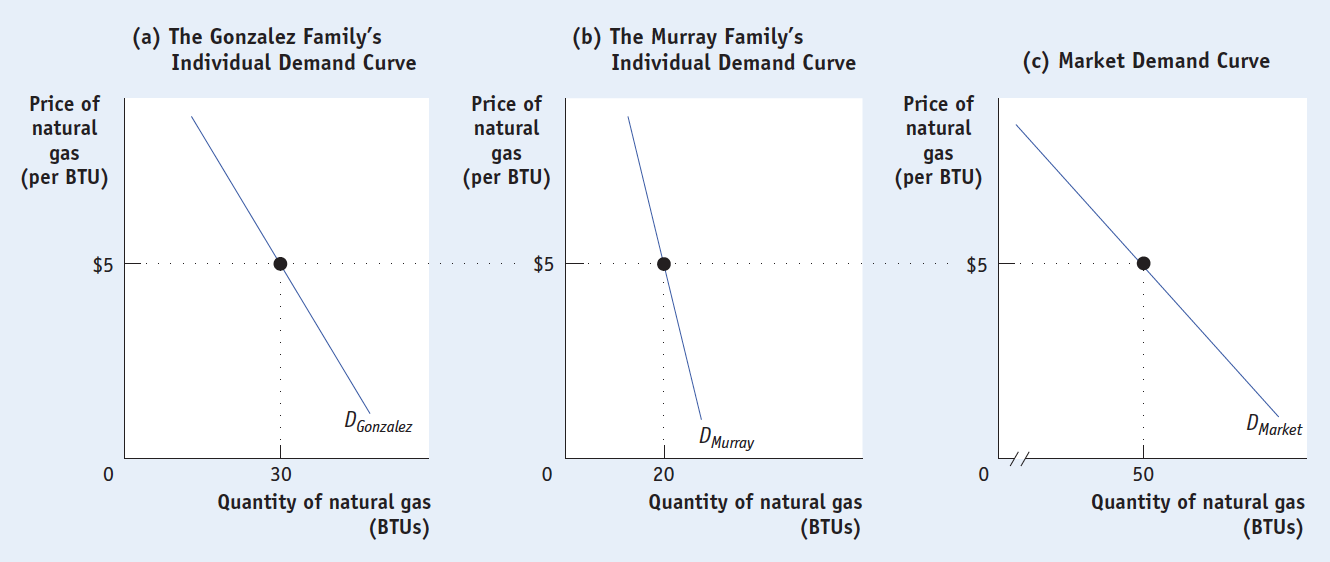
\includegraphics[width=\textwidth]{demandIndividual}
\end{figure}

	\end{enumerate}
	
	
		
\subsection{Supply Curve}

\lecture{18}{01}{2019}

\par{By considering the production of goods, instead of their consumption/demand, we get the analogous supply curve. Note that while the demand curve is in general decreasing (lower price $\implies$ more consumption), the supply curve is generally increasing. This makes sense, as \ita{all things equal}, higher pricers translate into higher profits}

\defn{Quantity Supplied}{Actual amount a producer would be willing to sell their products for a specific price}

\defn{Supply Schedule}{How much of a good or service producers will want to sell at different prices}

\defn{Supply Curve}{Graphical representation of the relation between quantity supplied and price}



\begin{figure}[ht]
\centering
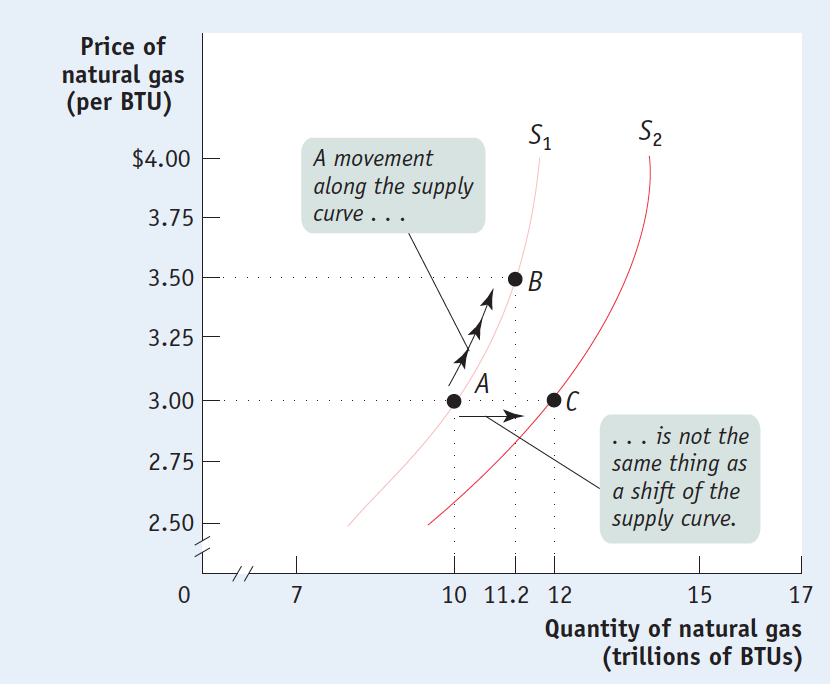
\includegraphics[width=0.5\textwidth]{supplyCurve}
\end{figure}

\par{Note that just like when looking at the demand curve, it's important not to confuse quantity supplied with supply, and their corresponding changes; a movement along the supply curve (increase in q.s) and a shift of the whole curve (increase in supply). The five major causes of a change in supply are due to changes in one or more of the following \textbf{non-price determinants}:}

\begin{enumerate}
	\item Input prices
	
	\defn{input}{good or service used to produce other goods/services}
	
	\par{The supply curve shifts inversely to the price of inputs, i.e. if an input becomes costlier, there's a reduction in supply $=$ shift to the left, and vice-versa}
	
	\item Prices of related goods or service
	
	\par{An increase in the price of a \ita{substitute} product will lead to a decrease in supply of its "pair" product. The reverse is true for its \ita{complement}.}
	
	\ex{If a company sells products A,B which serve roughly the same purpose, an increase of the price of A will make it more profitable, hence the company will decide to allocate more resources to A and decrease supply of B}

	\item Technology
	
	\par{Technological advancements lead to a decreased input cost, which in turn decreases the total cost of production leading to an increase in supply}
	
	\item Expectations
	
	\par{A producer may decide to store part of its goods to sell at a latter date, when demand is expected to be higher. This choice depends on a comparison of the current price versus the expected future price}
	
	\item Number of producers
	
	\par{Just like with the individual demand curve, if there are several producers of the same type of good, the supply curve will be equal to the horizontal sum of each producer's individual curve}
	
	\begin{figure}[ht]
\centering
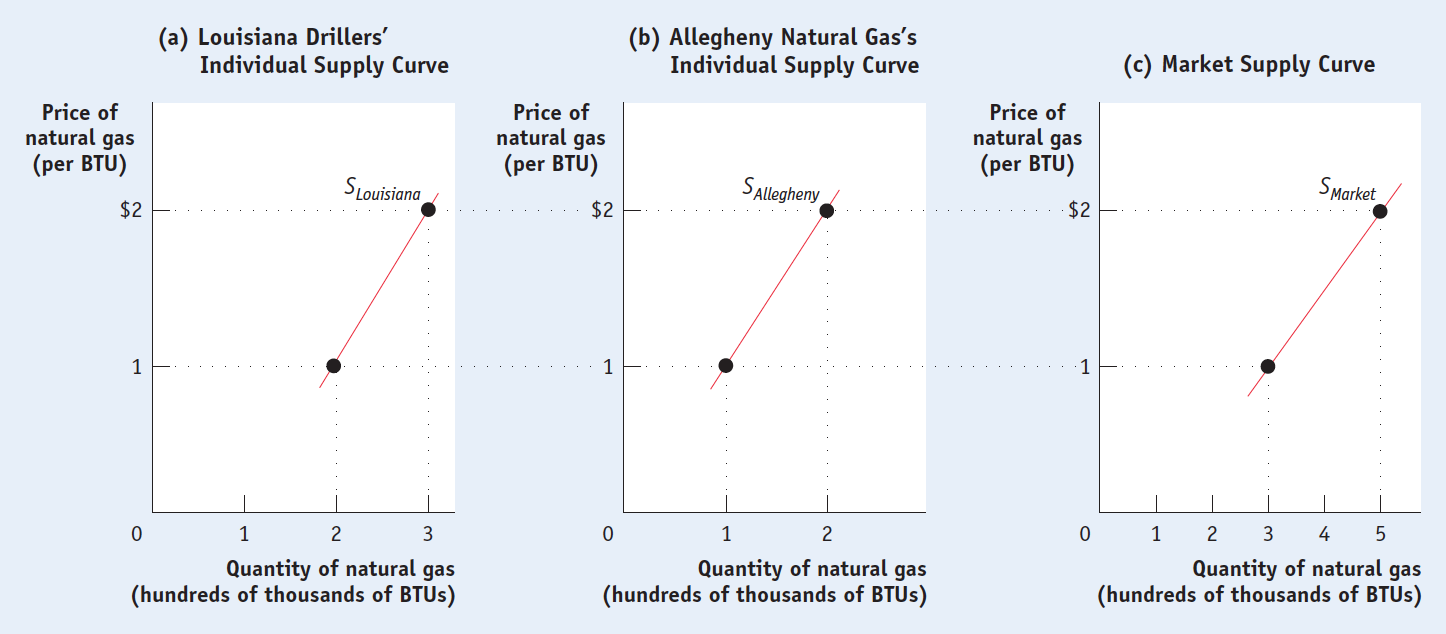
\includegraphics[width=0.5\textwidth]{supplyIndividual}
\end{figure}

\end{enumerate}

\subsubsection{Equilibrium}


\defn{Equilibrium Price*~\mymarginpar{*market clearing price}}{The price where the quantity demanded and supplied match.}

\rem{This is easily observed by finding the intersection of the supply and demand curves}

\par{In general, the market price will tend towards an equilibrium due to the following:}

\begin{enumerate}

\item Homogeneity

	\par{Given that both buyers and sellers are well informed of the "normal" prices in a certain area for a certain product, consumers will look for the cheaper products which achieve the same, or similar end. Sellers must have competitive prices (too low $\implies$ profit loss ; too high $\implies$ costumers loss)}
	
\item Price Fall

	\par{If the prices are set above that of the equilibrium, there will be a \ita{surplus} of goods. The market will adjust, by lowering the price towards eq}
	
	\defn{Surplus}{Quantity demanded $<$ Quantity Supplied}
	
\item Price Rise

	\par{If the prices are set below that of the equilibrium, there will be a \ita{shortage} of goods. The market will adjust, by raising the prices towards eq. so that quantity demanded is lowered}
	
\end{enumerate}


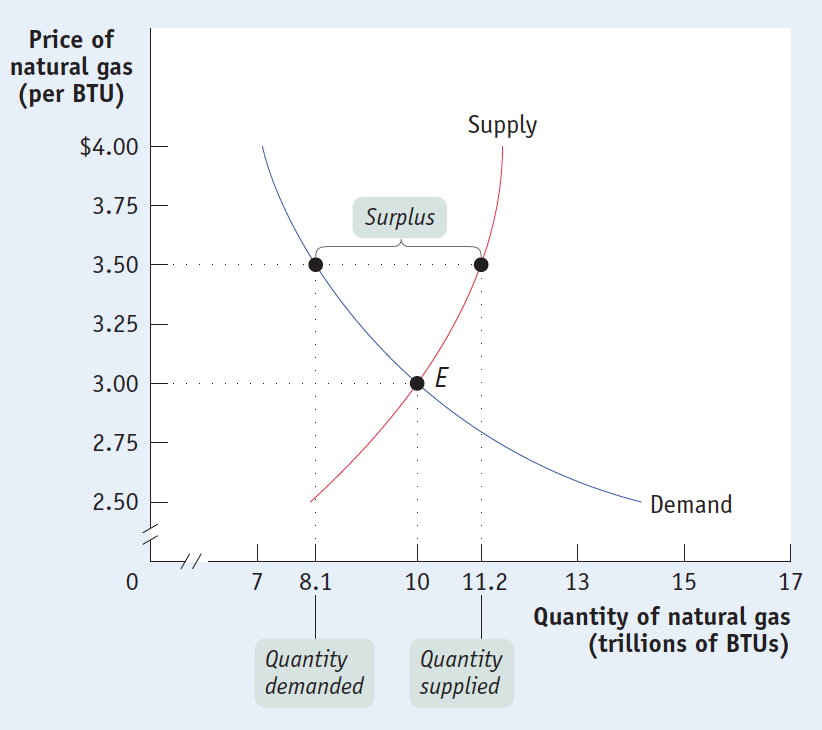
\includegraphics[width=15em]{supplySurplus}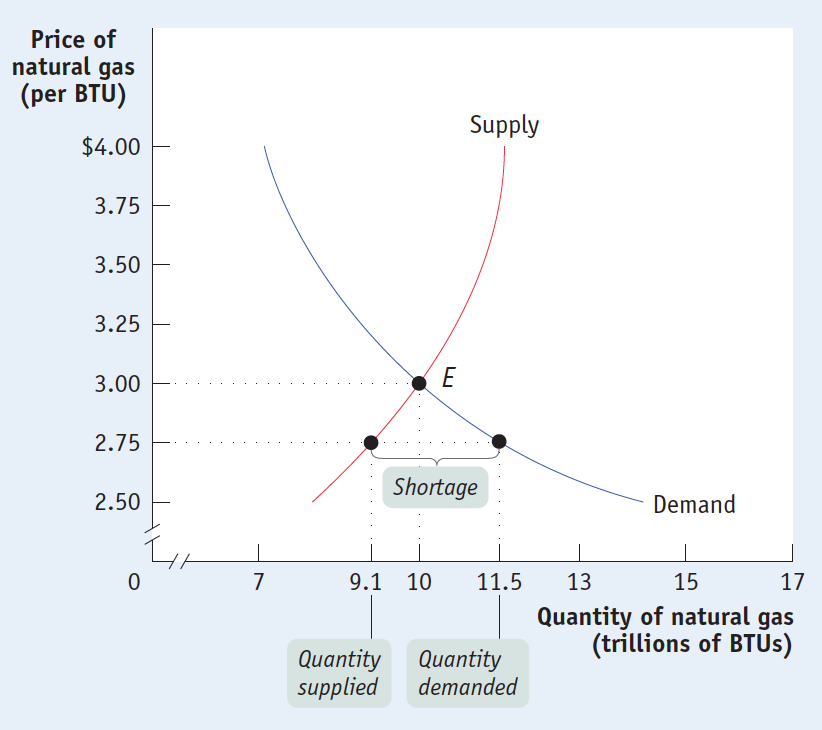
\includegraphics[width=15em]{supplyShortage}


	\par{Considering what happens to the equilibrium point when changes in supply and demand occur, one finds that:}
	
	\defn{Shortage}{Quantity Demanded $>$ Quantity Supplied}
	\begin{enumerate}
		\item An increase in demand leads to an upward movement along the supply curve, i.e. both the price and quantity demanded increase*~\mymarginpar{and vice-versa}
		\item An increase in supply leads to a downward movement along the demand curve, i.e. the price decreases while the demand increases*
	\end{enumerate}
	
	\rem{When there's a shift in both the demand and supply, if the price and quantity of equilibrium move together, then this is due do a change in demand. When they move in opposite directions, then it is due to a change in supply}

\begin{figure}[ht]
\centering
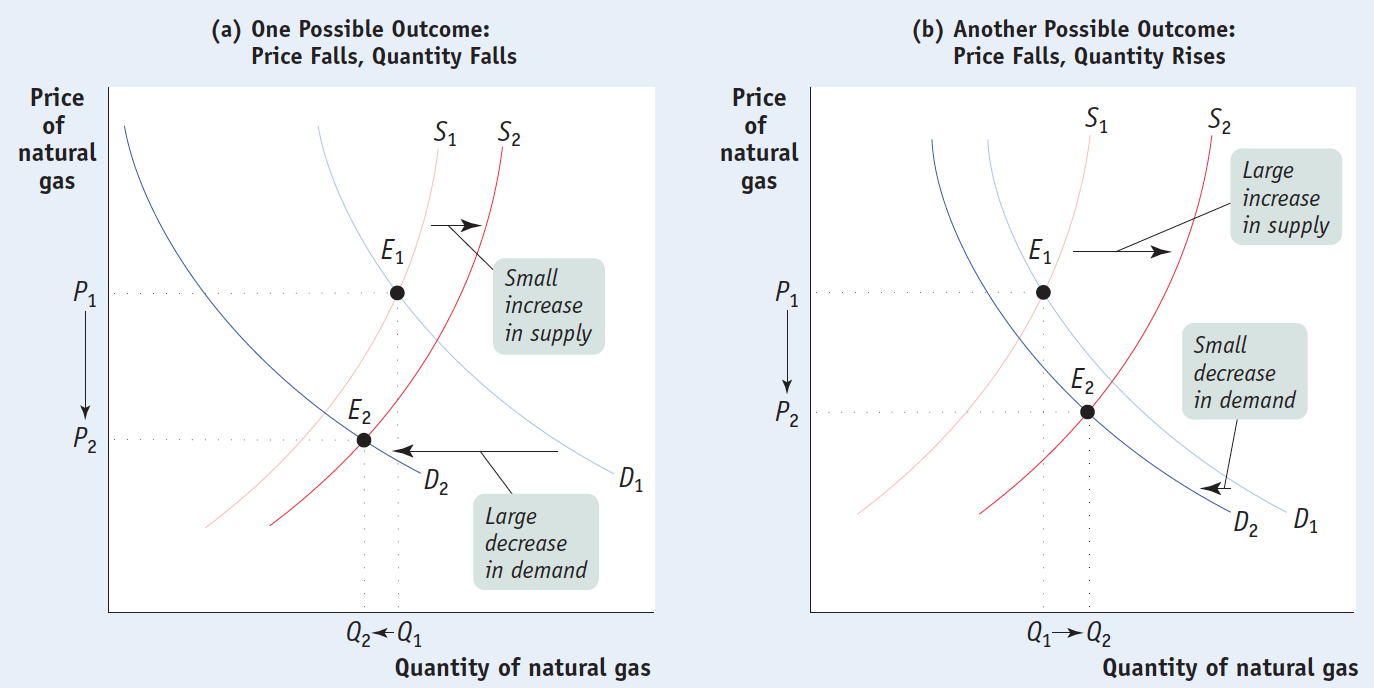
\includegraphics[width=\textwidth]{supplydemandEq}
\end{figure}

\newpage
\section{Consumer and Producer Surplus}

\lecture{22}{01}{2019}
\subsection{Consumer}

\defn{Willingness to Pay}{maximum price at which the buyer would buy the good}

\defn{Individual Consumer Surplus}{net gain to an individual buyer from a purchase}

\nota{  S = Willing - Actual}

\defn{Total Consumer Surplus}{net gain of all individuals}

\rem{Economists use consumer plus to mean both total and individual, it can be differentiated from context}


\begin{figure}[ht]
\centering
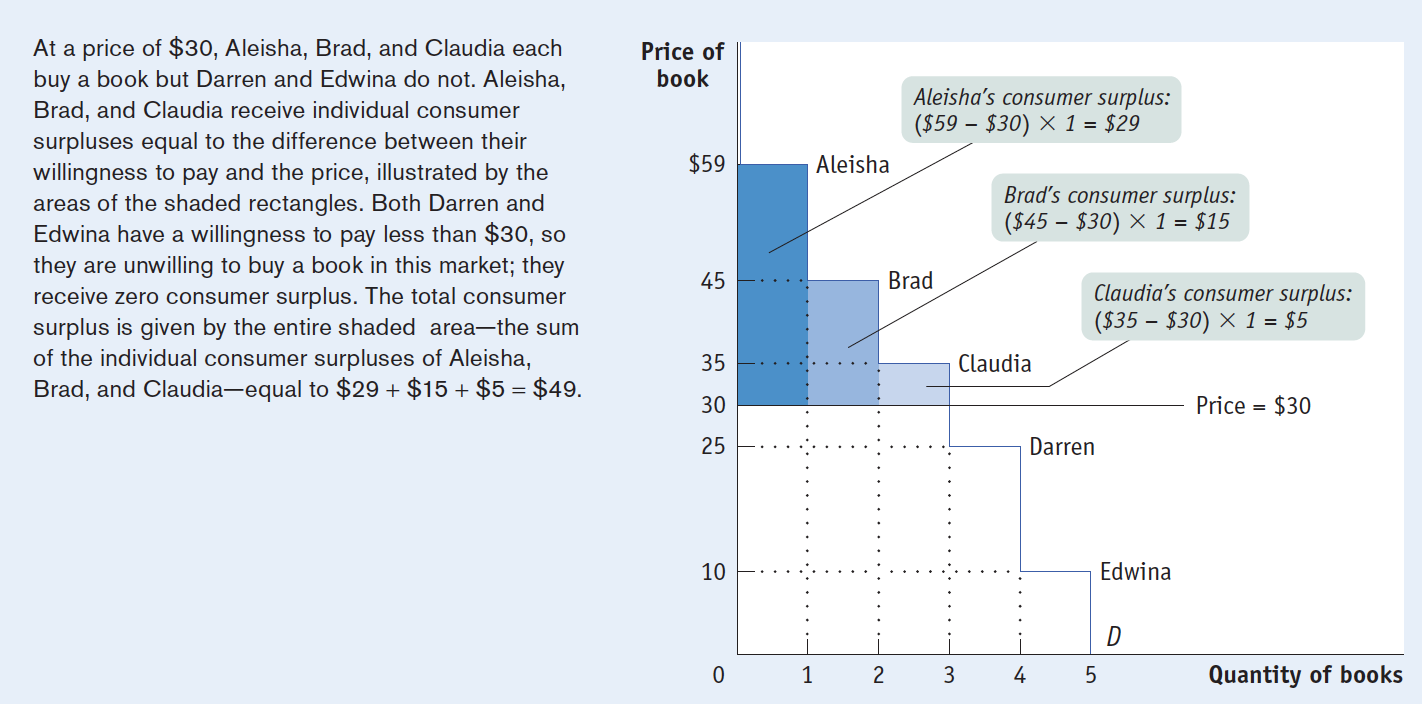
\includegraphics[width=0.7\textwidth]{consumerSurplus}
\end{figure}

\rem{It is intuitively obvious, that a change in market price varies inversely with consumer surplus}

\subsection{Producer}

\par{The producer surplus works much in the same way, but in reverse. The gains for sellers are calculated by looking at the difference between the min price a seller would be willing to sell his products/goods and the actual price it was sold}

\defn{Cost}{the lowest price at which he or she is willing to sell a good}

\defn{Individual Producer Surplus}{net gain to an individual producer from a sale}

\defn{Total Producer Surplus}{net gain of all individual producers}

\begin{figure}[ht]
\centering
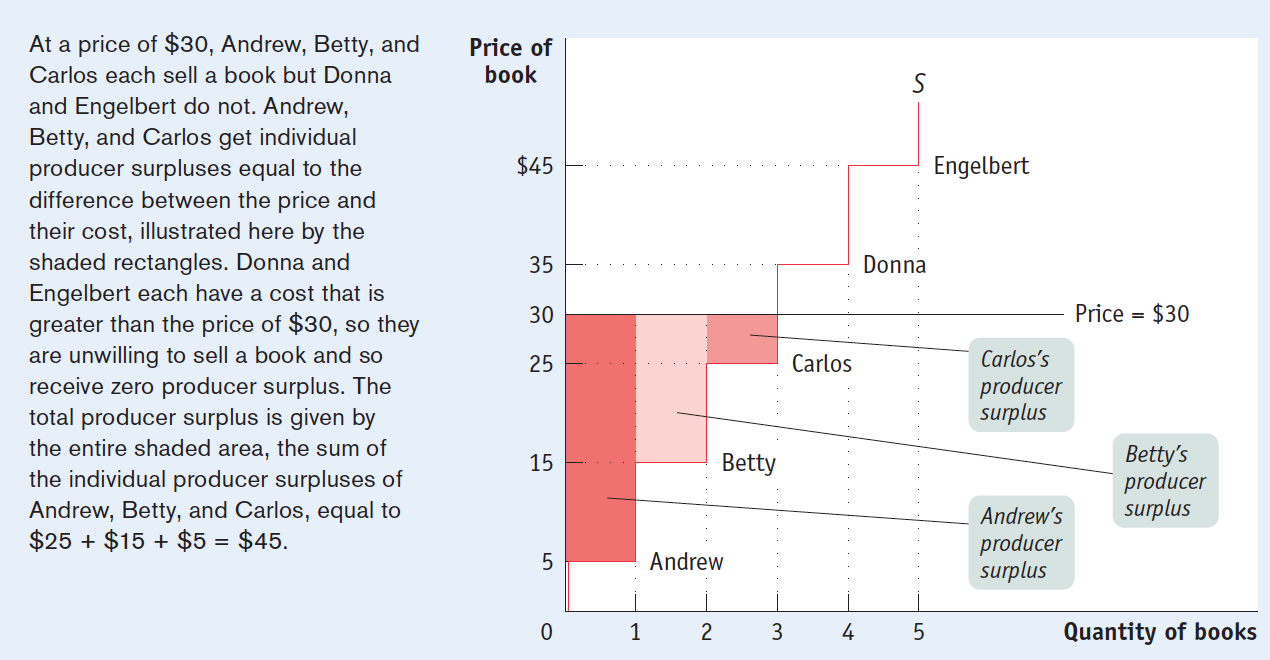
\includegraphics[width=0.7\textwidth]{producerSurplus}
\end{figure}

\rem{Once again it should be obvious that if the market price increases the producer surplus will also increase}

\par{By looking at the net gains generated for both producers and consumers we can calculate the total surplus for a market. This is evidence that trade can be beneficial for both}

\defn{Total Surplus}{the sum of the producer and consumer surplus}

\begin{figure}[ht]
\centering
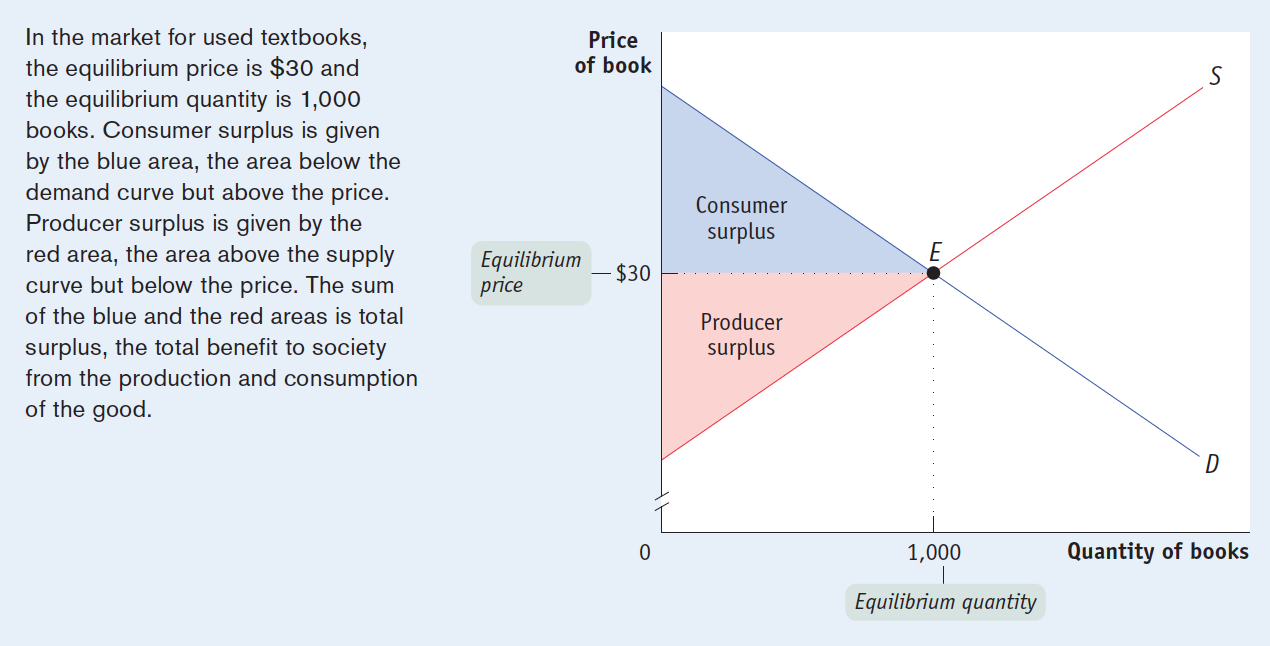
\includegraphics[width=0.7\textwidth]{CPsurplus}
\end{figure}


\rem{The surplus is the area found below (producer) and above (consumer) the equilibrium price}


\subsection{Efficiency}


\par{We can analyse the efficiency of a market in the light of consumer and producer surplus. Say for example that one is aiming to improve the market equilibrium by increasing total surplus. How could this be achieved? In essence an efficient market performs the following four functions:}

\begin{enumerate}
	\item It Allocates consumption of the good to the potential buyers who have the highest willingness to pay.
	
	\item  It allocates sales to the potential sellers who most value the right to sell the good, as indicated by the fact that they have the lowest cost.
	
	\item It ensures that every consumer who makes a purchase values the good more than every seller who makes a sale, so that all transactions are mutually beneficial.
	
	\item It ensures that every potential buyer who doesn't make a purchase values the good less than every potential seller who doesn't make a sale, so that no mutually beneficial transactions are missed.
\end{enumerate}

\par{In general, \ita{any way of allocating the good other than the market equilibrium outcome lowers total surplus}. There is however things one must watch out for when relying purely on markets.}

\begin{enumerate}
	\item Equity/Fairness is often in conflict with efficiency: As a society we often don't think as efficiency as the only goal to be achieved, in fact most modern societies understand the trade-off between the two, and often prize the distribution of wealth over the maximisation of efficiency. The reason why this two conflict is that efficiency deals only with maximising a the output of a function given certain inputs, once the output/goal being optimised is defined that's what the optimising strategies will work to increase regardless of what extraneous consequences it might have
	
	\item Markets Fail: 
		\begin{itemize}
		\item in an attempt to capture more surplus, one party prevents mutually beneficial trades from occurring (monopoly)
		\item actions of individuals sometimes have side effects*~\mymarginpar{externalities e.g. pollution} on the welfare of others that markets don't take into account
		\item Markets for some goods fail because these goods, by their very nature, are unsuited for efficient management by markets. (e.g. problems of private information - used car)
		\end{itemize}
		
	\item Even when the market equilibrium maximizes total surplus, this does not mean that it results in the best outcome for every individual consumer and produce
\end{enumerate}

\par{When markets are efficient, the economy as a whole is efficient. Even though economies where every market is efficient are a theoretical construct, some are much more efficient than others. Why is that? It all comes down to two main market features (1) Property Rights; (2) Prices as Economic Signals }

\defn{Property Rights}{system in which valuable items in the economy have specific owners who can dispose of them as they choose}

\par{By taking ownership full ownership of goods once bought, this reduces the opportunity-cost of the item. For example, by knowing in advance that I might be able to sellback a textbook which I only need for a semester, I will in recoup part of its original cost, and the student buying it will not only be able to buy it at a reduced cost, but will also gains the right to resell it} 

\defn{Economic Signals}{any piece of information that helps people and businesses make better economic decisions}

\par{Business analysts often know that a business is preparing to ramp production when it increases its purchase of cardboard boxes, we say that the boxes are a signal of changes in industrial production. In a more general case, prices in a market economy perform a similar function. By setting the market price of a good at $x$ , economic agents can derive useful information from  it. Sellers know that there are consumers willing to pay at least $x$, and consumers know that there are potential sellers with a cost of $x$ or less. The signal given by the market price ensures that total surplus is maximized by telling people whether to buy, sell , or do nothing at all.}

\rem{ Note that since, in equilibrium, the quantity demanded equals the quantity supplied, all willing consumers will find willing sellers.}

\rem{There are markets where prices are not a good economic signal, for example when there is uncertainty about the quality of a good. This is a well-known problem in economics know as \ita{"the market for lemons"}}

\section{Meddling with Markets}

\lecture{24}{01}{2019}

\par{There is often the need for the government to implement price controls, this can come in the form of price floors or price ceiling}

\subsection{Price Ceiling}

\defn{Price Ceiling}{government mandated maximum price at which a good can be sold}

\par{Price ceilings are often set in place during times of crises, where demand for certain goods sky-rockets, and producers tend to take advantage of the situation by charging way above market-price. However, when balanced markets are over-regulated predictable negative consequences arise, the main one being that producers seeing their profit margins decline tend to reduce supply, which leads to shortages. }

\rem{If the price ceiling is set above market price, we say that it is \ita{non-binding}, i.e. it will not constraint market behaviour}

\begin{figure}[ht]
\centering
\includegraphics[height=0.3\textwidth, width=0.5\textwidth]{ceilling}
\end{figure}


\begin{itemize}
	\item \textbf{Negative Consequences}
	\begin{enumerate}
		\item Low Quantity: given that producers will produce less, it necessarily follows that consumers will buy less. This mutual loss is called \ita{deadweight loss}, it represents the reduction in the total surplus.
		
		\defn{deadweight loss}{the loss in total surplus that occurs whenever an action or a policy reduces the quantity transacted below the efficient market equilibrium quantity}
		
		\begin{figure}[h]
\centering
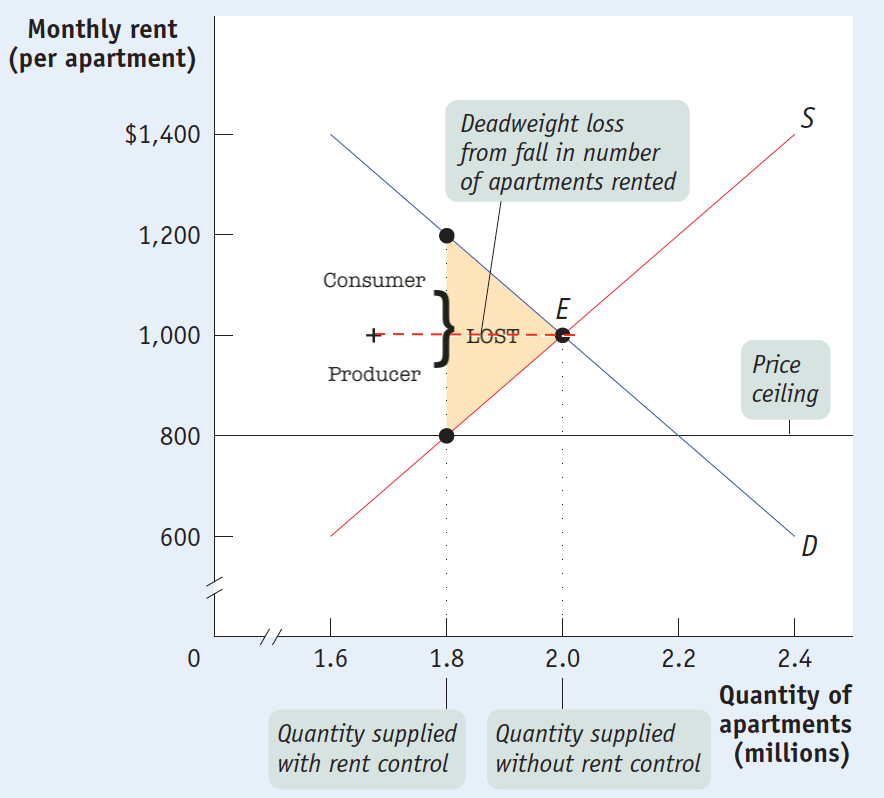
\includegraphics[height=0.4\textwidth,width=0.8\textwidth]{deadweight}
\end{figure}
\begin{figure}[h]
\centering
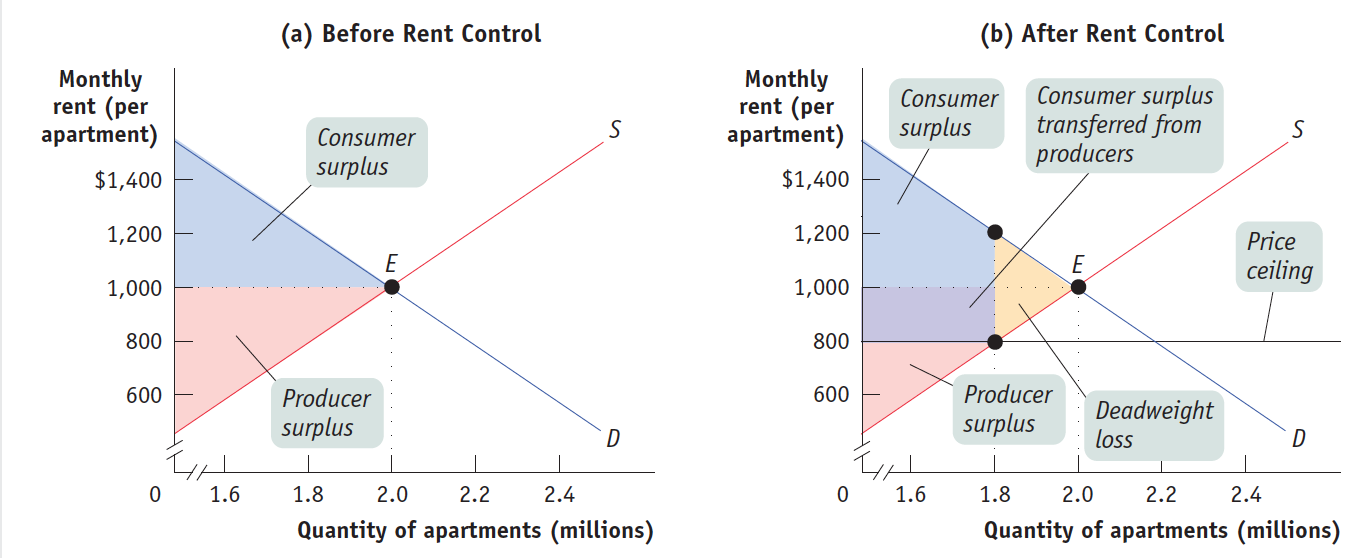
\includegraphics[height=0.4\textwidth,width=0.8\textwidth]{deadweight2}
\end{figure}
	
	\item Allocation to Consumers: apartment, some want one badly and are willing to pay a high price to get it. Others have a less urgent need and are only willing to pay a low price~\mymarginpar{Krugman correlates willing max price to urgency/necessity, but it doesn't necessarily follow! One might be in dire need of a house, but simply not be able to afford to go any higher}. By "lowering the bar" for everyone, other factors other than price (personal connections, luck) will take over the allocation, which often turns out to be inneficient
		
	\item Wasted Resources: people expend money, effort, and time to cope with the shortages caused by the price ceiling
	
	\item Low Quality: sellers offer low-quality goods at a low price even though buyers would rather have higher quality and would be willing to pay a higher price for it
	
	\item Black Markets
	
	\end{enumerate}
	
	\item \textbf{Why are ceilings needed?} \par{they give a small minority
of buyer much cheaper products than they would get in an unregulated market, which they wouldn't otherwise be able to afford}

\end{itemize}

\subsection{Price Floors}


\defn{Price Floor}{government mandated minimum price at which a good can be sold (e.g. min wage)}

\par{Price floors are often set in place as an aid to highly competitive  markets (e.g. job market, farming), where supply for certain goods is plenty.}

\begin{figure}[h]
\centering
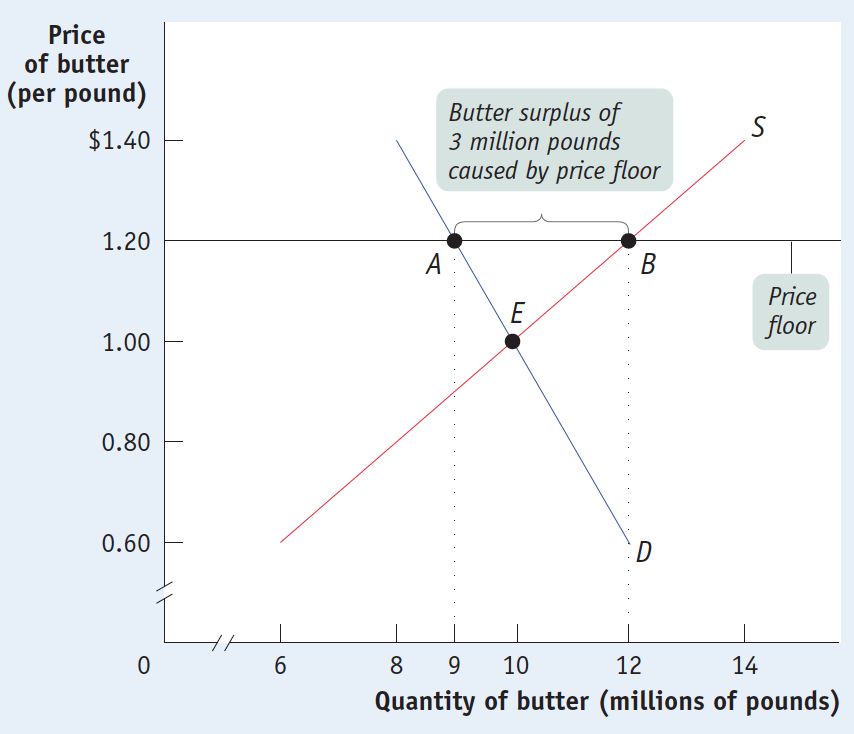
\includegraphics[width=0.5\textwidth]{floor}
\end{figure}

\rem{Both ceilings and floors have the effect of reducing the quantity of a good bought and sold. When the quantity of a
good supplied isn't equal to the quantity demanded, \textbf{the actual quantity sold is determined by the "short side" of the
market (whichever quantity is less)}. Sellers don't want to sell as much as buyers want to buy, it's the sellers who determine the actual quantity sold. If buyers don't want to buy as much as sellers want to sell, it's the buyers who determine the actual quantity sold}

\rem{The negative side effects are similar to those of price floors}

\subsection{Controlling Quantities}
\lecture{25}{01}{2019}

\par{Until now we have been focusing on government intervention on the prices of goods, in this section we'll focus on controlling quantities}

\defn{Quota}{an upper limit on the quantity of
some good that can be bought or
sold.}

\defn{Quota Limit}{the total amount of the good
that can be legally transacted}

\rem{This limits are usually enacted by issuing licenses, which limits the number of people which can sell the good}

\defn{Demand Price}{the price at which
consumers will demand that quantity.}

\defn{Supply Price}{the price at which producers will
supply that quantity.}

\par{Licenses are not free, the owner of a licence must buy it from the local council, which makes it in itself a commodity separate of the good. Therefore, when analysing transactions one must consider two distinct (but related) markets (1) the transactions between customer-seller (2) transactions of licenses.}
\par{Given that this cost of the license is usually carried over to customers, there is a a difference between what  customers pay and the profit the seller does, this difference can be see as the license fee which belongs to the license holder who usually leases it}

\defn{wedge}{a difference between the demand price
and the supply price of a good; that
is, the price paid by buyers ends up
being higher than that received by
sellers.}

\defn{quota rent}{the earnings that
accrue to the license-holder from
ownership of the right to sell the
good. It is equal to the market price
of the license when the licenses are
traded.}

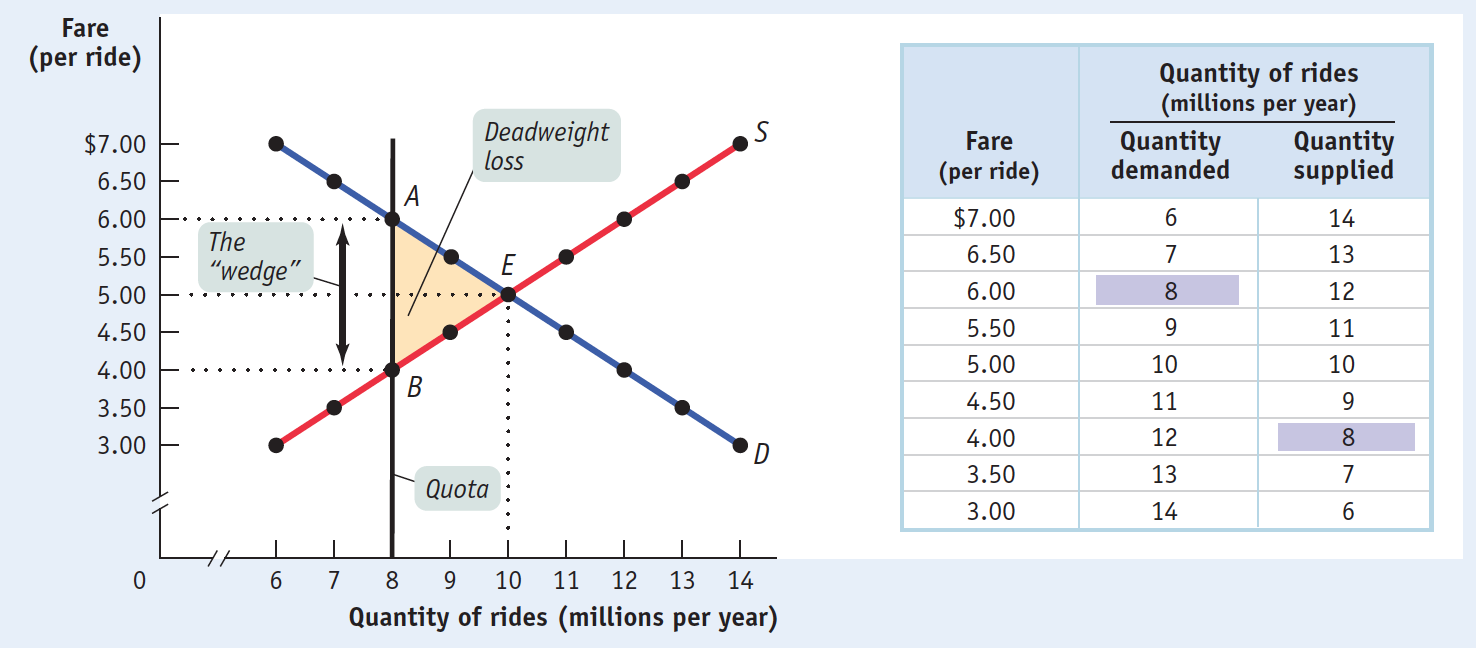
\includegraphics[width=\textwidth]{control}

\newpage

\section{Elasticity}


\defn{Elasticity}{a measure of a variable's sensitivity to a change in another variable}

\defn{Price Elasticity of Demand}{change in the quantity demanded in relation to a price change}

$$ PED = \left|\frac{\% \ \Delta QD}{\% \ \Delta P} \right|$$

\rem{remember to change the change to a percent value}

\rem{Due to (\ref{demand:law}) , the value will always be negative, indicating that QD and P vary inversely. By convention the sign is dropped}

\defn{Elastic}{A product $P$ is deemed to be elastic, if its $PED < 1$; i.e if the change in price is greater than the change of the quantity demanded}

\defn{Inelastic}{$PED > 1$; change of qd is greater than price change}

\defn{Unit Elastic}{$PED = 1$}

\par{\textbf{The Midpoint Method} is used , instead of the method above, to avoid computing different elasticities for different pov's. For example, John is 180cm tall and Mary is 162cm tall. From John's perspective, their percentual difference is 110\% while from Mary's is 90\%} \TODO{Ask! if they vary by 10, when using the words taller/shorter than this is assumed. So why is it necessary}

\par{The concept is still the same but the change of the variables is divided by its average}
\ex{
$$ \% \Delta QD = \frac{QD_2 - QD1}{\sfrac{(QD_2 + QD_1)}{2}}$$
}

\par{In general:}

$$ \% PED = \frac{\tfrac{QD_2 - QD1}{\sfrac{(QD_2 + QD_1)}{2}}}{\tfrac{P_2 - P1}{\sfrac{(P_2 + P_1)}{2}}}$$

\subsection{Interpreting PED}

\defn{Perfectly Inelastic}{changes in price do not affect the quantity demanded}

\par{Note that in the case where customers do not respond to changes in price (e.g. serious chronic disease medication), the demand curve will in fact just be a vertical line, since $\Delta QD = 0$}

\defn{Perfectly Elastic}{changes in demand do not affect price}

\par{Note that in the case where \ita{any} price change leads to extreme changes in the quantity demanded*\mymarginpar{*real life scenarios are scarce, but a close example would be of two products which are really good substitutes of each other}, the demand curve will then be an horizontal line, since for $+\Delta P , \Delta Q \to 0$ and  $-\Delta P, \Delta Q \to \infty$} \TODO{ASK! Should there not be two asymptotes instead of a horizontal line?}

\rem{Note then that in general, since we represent price in the $y$ axes and qd in the $x$ axes, $PED = \frac{1}{\frac{dy}{dx}}$ , it follows then that the steeper the gradient , the less elastic a product is}


              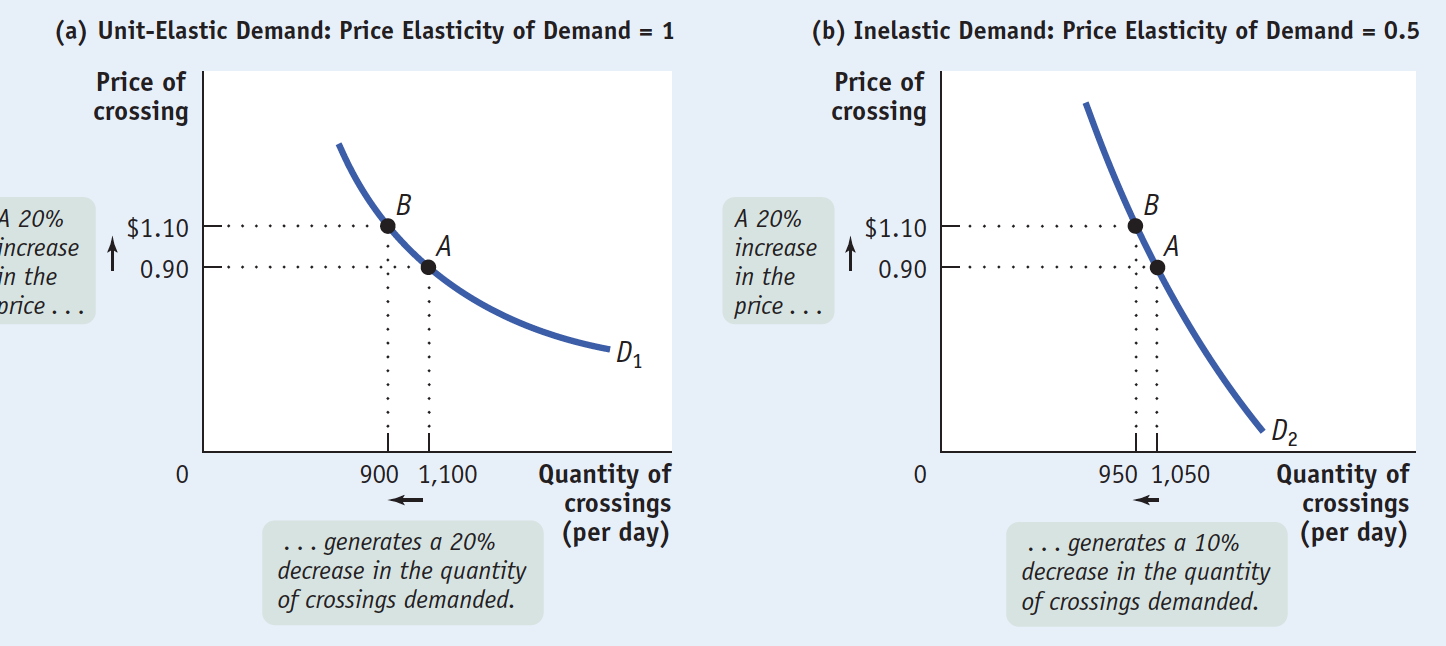
\includegraphics[width=0.65\linewidth]{elasticGrad} 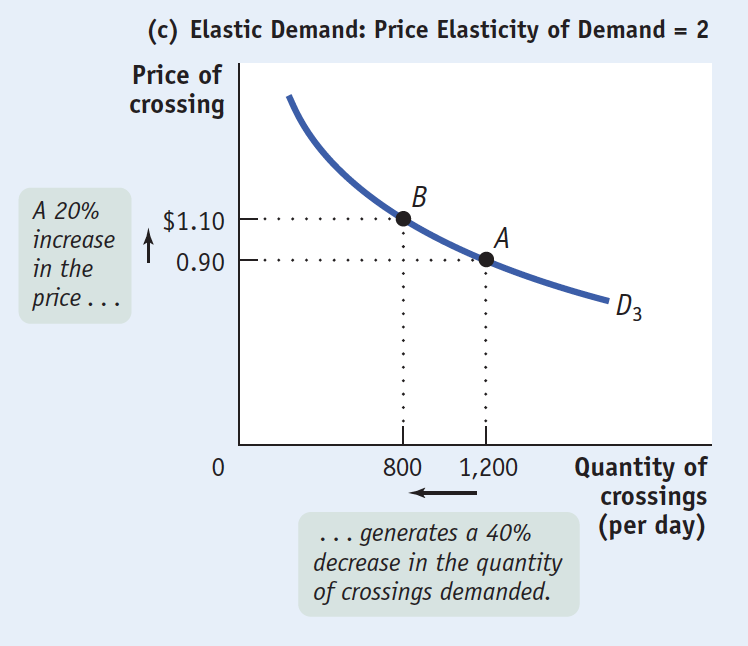
\includegraphics[width=0.335\linewidth]{elasticGrad2}

\par{The notion of elasticity is obviously useful to predict how of possible changes in price will affect the \ita{total revenue}.}

\defn{Total Revenue}{the total value of sales of a good, equal to the price multiplied by the quantity sold}

$$T_n = P_n \cdot Q_n$$ 

\par{where $T_n$ represents the total revenue of a good at the point $(Q_n,P_n)$ in the demand curve\\}

\par{The total revenue after a change can still be calculated in the same way. We should expect the area to change due to the (1) price effect ; (2) demand effect. It should be intuitively obvious that by raising the price the p/product revenue will be higher, and the opposite is true when reducing quantities. However, the elasticity of the curve is useful to help us understand which of these effects will be stronger, and in turn what happens to the \ita{net total revenue}}

\par{It is useful again to think of the gradient of the curve and the area of the rectangle strictly below the point we're looking at. Note the following for a price increase along the curve\mymarginpar{obviously the opposite is true for a decrease}:} 

\begin{itemize}
	\item{\textbf{Elastic:} for a steeper gradient, even a small decrease in qd will result in a very large increase in price (think of an exponential curve). Hence, \textbf{the revenue lost by the lost units will be compensated by the revenue gained by the increase in price}}
	\item{ \textbf{Non-Elastic:} the opposite}
	\item{ \textbf{Unit-Elastic:} still no change}
\end{itemize}

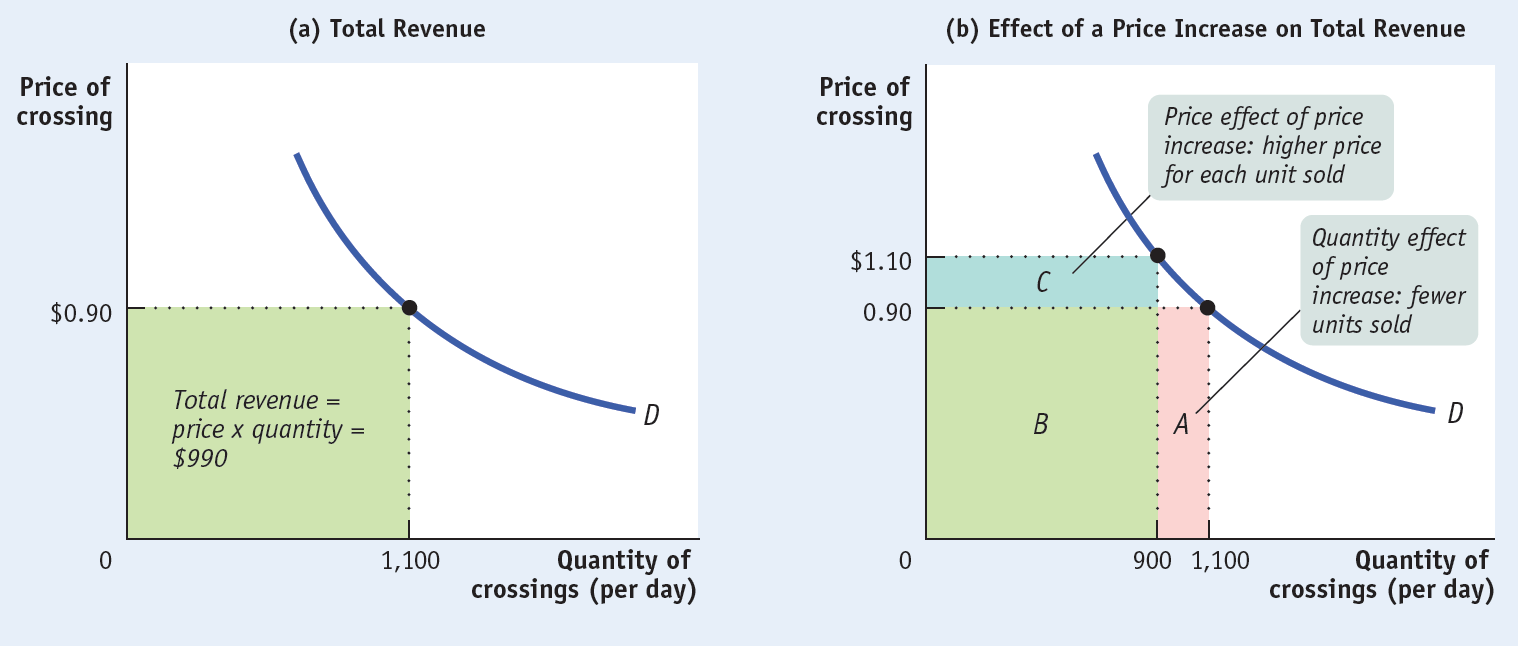
\includegraphics[width=\linewidth]{elasticRev}

\rem{Price elasticity varies along the curve}

\par{Given that the demand curve has a negative gradient, and following from the analysis above, the following are true:}

\rem{If the price between two points $x_1 , x_2$ decreases and the total revenue increases, then $x_1$ is \ita{more elastic} than $x_2$, \textbf{but} both prices are elastic}

\rem{f the price between two points $x_1 , x_2$ decreases and the total revenue decreases, then $x_1$ is \ita{less elastic} than $x_2$ \textbf{but} both prices are non-elastic}

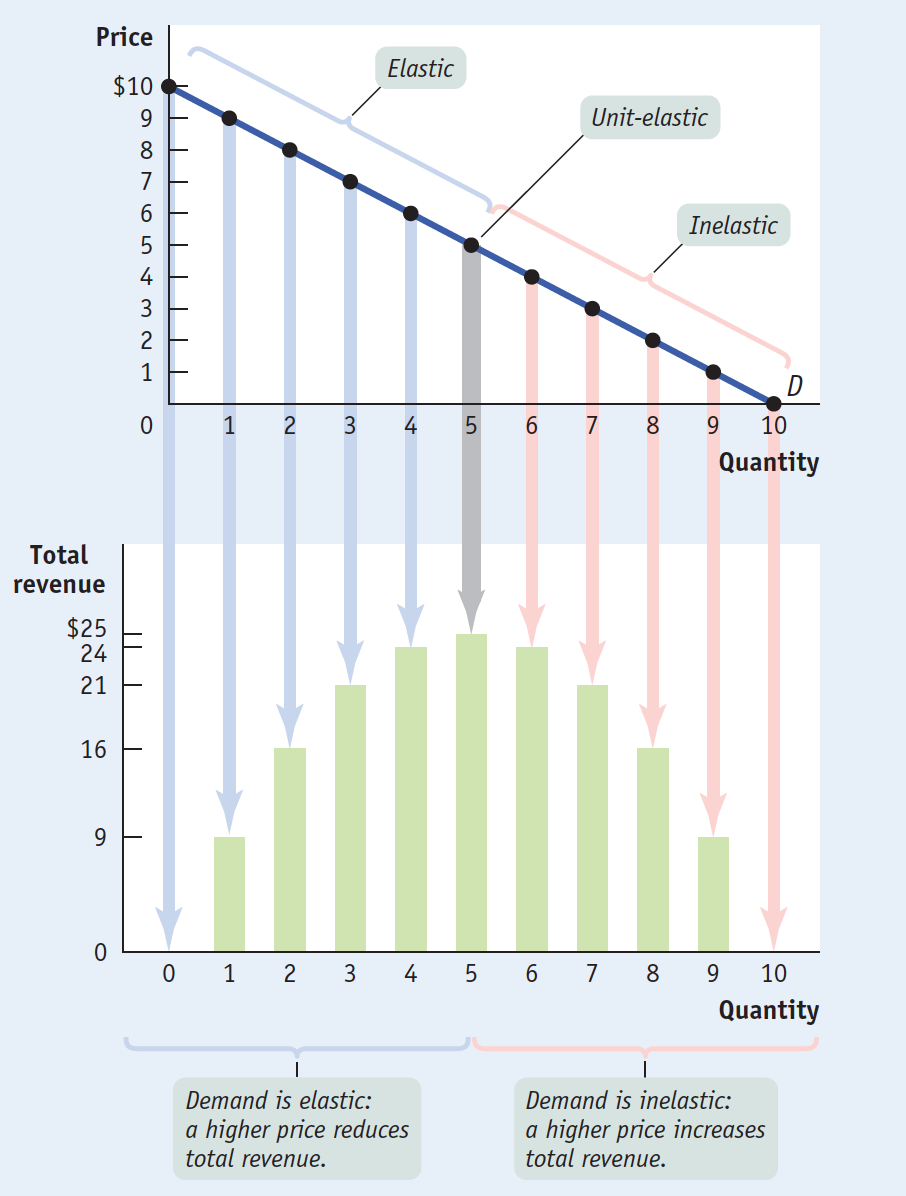
\includegraphics[height=0.8\linewidth, width=0.7\linewidth]{elasticVar}


\rem{The revenue maximum occurs when demand is unite-elastic}

\subsubsection{Factors of Influence}

\begin{enumerate}
	\item Luxury Vs Necessary Goods
	\par{Luxury goods tend to be much more elastic, since people can "live without them" which wither forces sellers to reduce the price or the quantity demanded is low}
	\item Availability of Close Substitutes
	\par{If there are close substitutes for a good, its price elasticity will be higher, again because people have choices}
	\item Share of Income Spent
	\par{ If people spend a large chunk of their income in a good, they don't mind spending time finding ways to reduce its quantity demanded, hence higher elasticity}
	\item Time Since Price Change
	\par{ Elasticity tends to increase with time}
\end{enumerate}

\subsection{Other Demand Elasticities}

\par{The quantity demanded of a good depends on variables other than price, we can study this variation with other elasticities}

\defn{Cross-Price}{measures the effect of the change in one good's price on another's quantity demanded

$$CP_{ab} =\% \frac{\Delta QD_{a}}{\Delta P_{b}}$$}

\rem{$a , b$ substitutes $\implies CP_{ab} > 0 \implies$ right shift of the D curve}

\defn{Income Elasticity}{measures the effect of a change in consumers' income on a good's demand
$$IED =\% \frac{\Delta QD}{\Delta I}$$}

\rem{Useful to understand if a good is inferior or normal}

\rem{If $IED > 0 \implies $ normal good}


\subsection{Price Elasticity of Supply}

\defn{Price Elasticity of Supply}{change in the quantity supplied in relation to a price change}

\subsubsection{Factors of Influence}

\begin{enumerate}
	\item Availability of Inputs
	\par{Elasticity tends to be large when inputs are readily available and can be shifted into and out of production at a relative low cost}
	\item Time
	\par{Elasticity grows larger as producers have more time to respond to price changes}
\end{enumerate}

\subsection{Elasticity Summary}
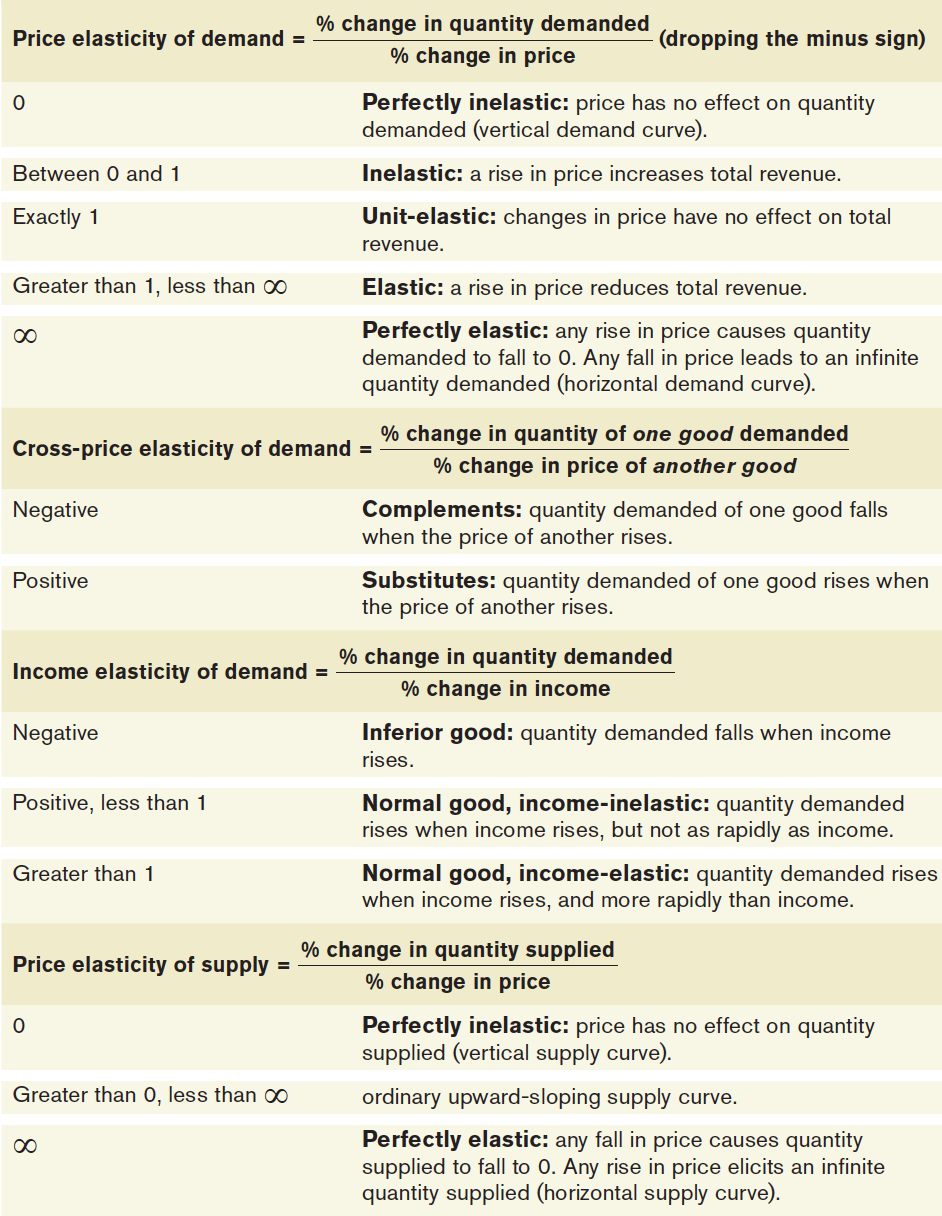
\includegraphics[height=1.1\textwidth]{elasticSum}
 
 \newpage
 
 \section{Taxes} 
\lecture{31}{01}{2019}

\defn{Excise Tax}{a tax charged on each unit of a good or service that is sold}

\par{Taxes have effects similar to those of quotas above. By imposing a tax on a good, the producer will tend to pass its costs onto the consumer. This will make goods in general more expensive, which in turn decreases demand.}
\par{So, \ita{for any given quantity} the amount producers are willing to charge is equal to that of Original Price + Tax. Which leads the supply curve to \ita{shift upwards by the tax amount}}

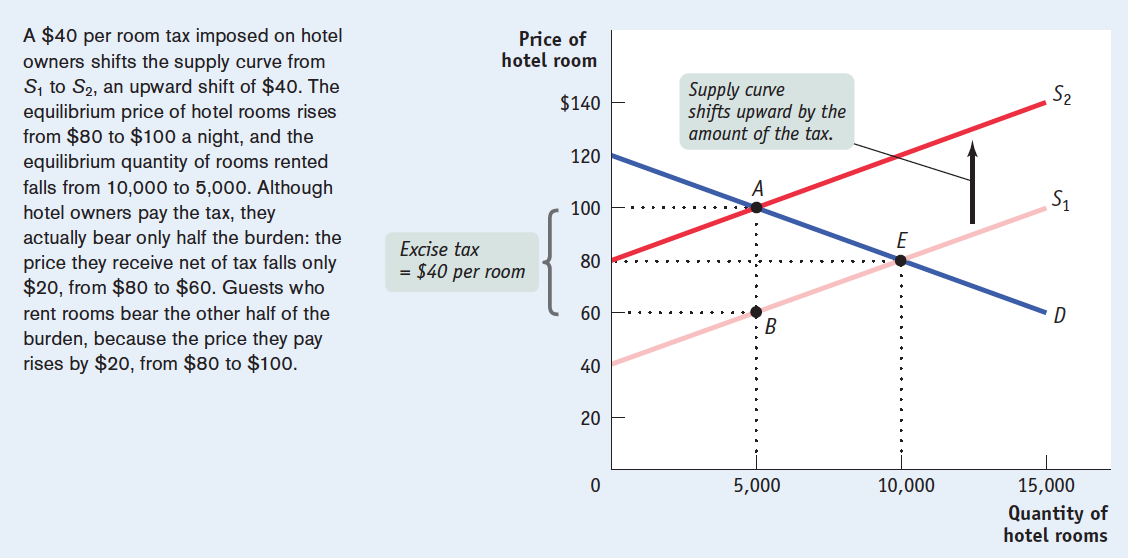
\includegraphics[width=\textwidth]{tax1}

\par{Note that in the example above, the consumers are paying 20\$ more than the original price, hence they are in effect paying half of the tax.}

\rem{Taxes can also be imposed on consumers, in which case the demand curve would be the one shifting. It would  of course shift downwards, since higher prices imply less demand}

\par{Note that regardless of who the tax is being imposed on, when looking at the same quantity (e.g. 5000), the guests pay in effect 100\$ and consumers 60\$}

\subsection{Incidence of a Tax}

\par{In the example above we've derived the \ita{general principle} that the outcome of taxation is the same regardless of who pays it. What is not necessarily true, is that the tax is always split 50-50. We can analyse the incidence of a tax by looking at price elasticity of supply and demand.}

\begin{itemize}
	\item[] Consumers: When the PED is low and the PES is high. This is because low PED $\implies$ few substitutes $\implies$ less flexibility. The reverse is true for supply, hence producers can use their "spare" goods for other purposes
	\item[] Producers: When the PED is low and the PED is high. This is because low PES $\implies$ few substitutes $\implies$ less flexibility. The reverse is true for demand, hence consumers can opt for similar goods.
\end{itemize}

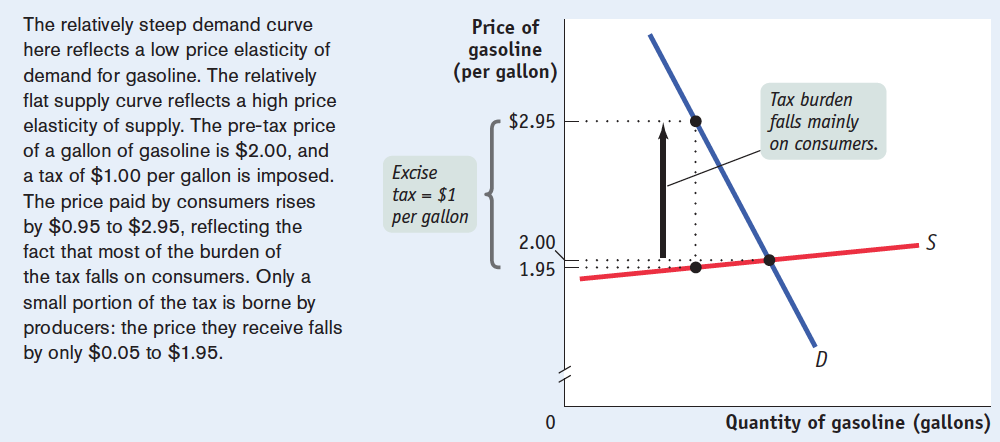
\includegraphics[width=\textwidth]{tax2} 
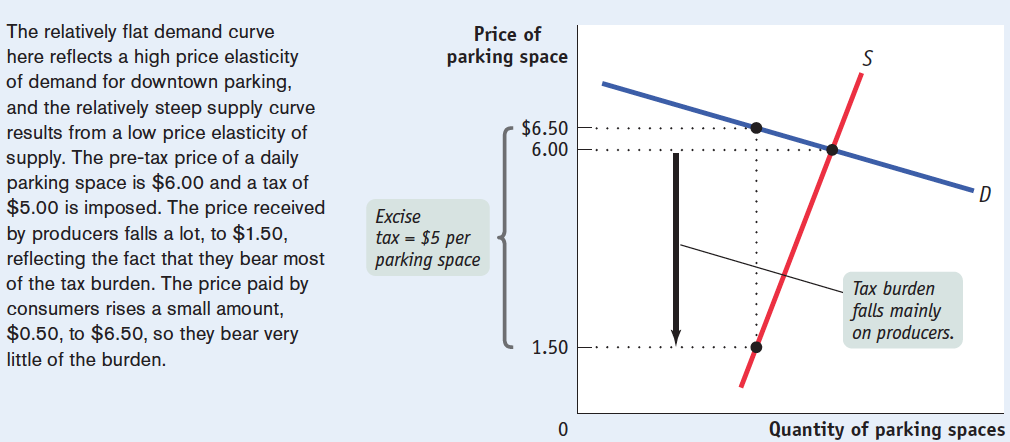
\includegraphics[width=\textwidth]{tax3} 

\subsection{Benefits and Costs of Taxation}

\par{The revenue collected from imposing a tax can be calculated by looking at the area of the triangle with height equal to the tax amount.\mymarginpar{look at quotas examples, for more a detailed analysis}. Once again, the net effect of raising a tax will depend on the elasticity of the curves.}

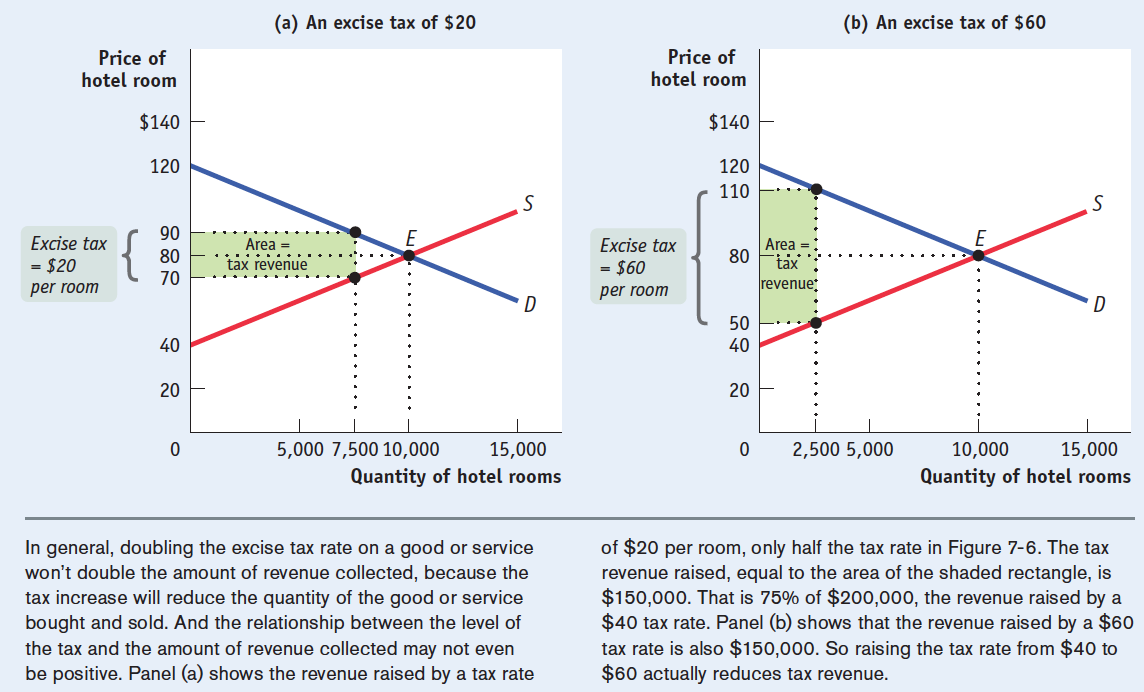
\includegraphics[width=\textwidth]{tax4}

\par{Given that the tax creates surplus, its costs are given by the \ita{deadweight loss} triangle}

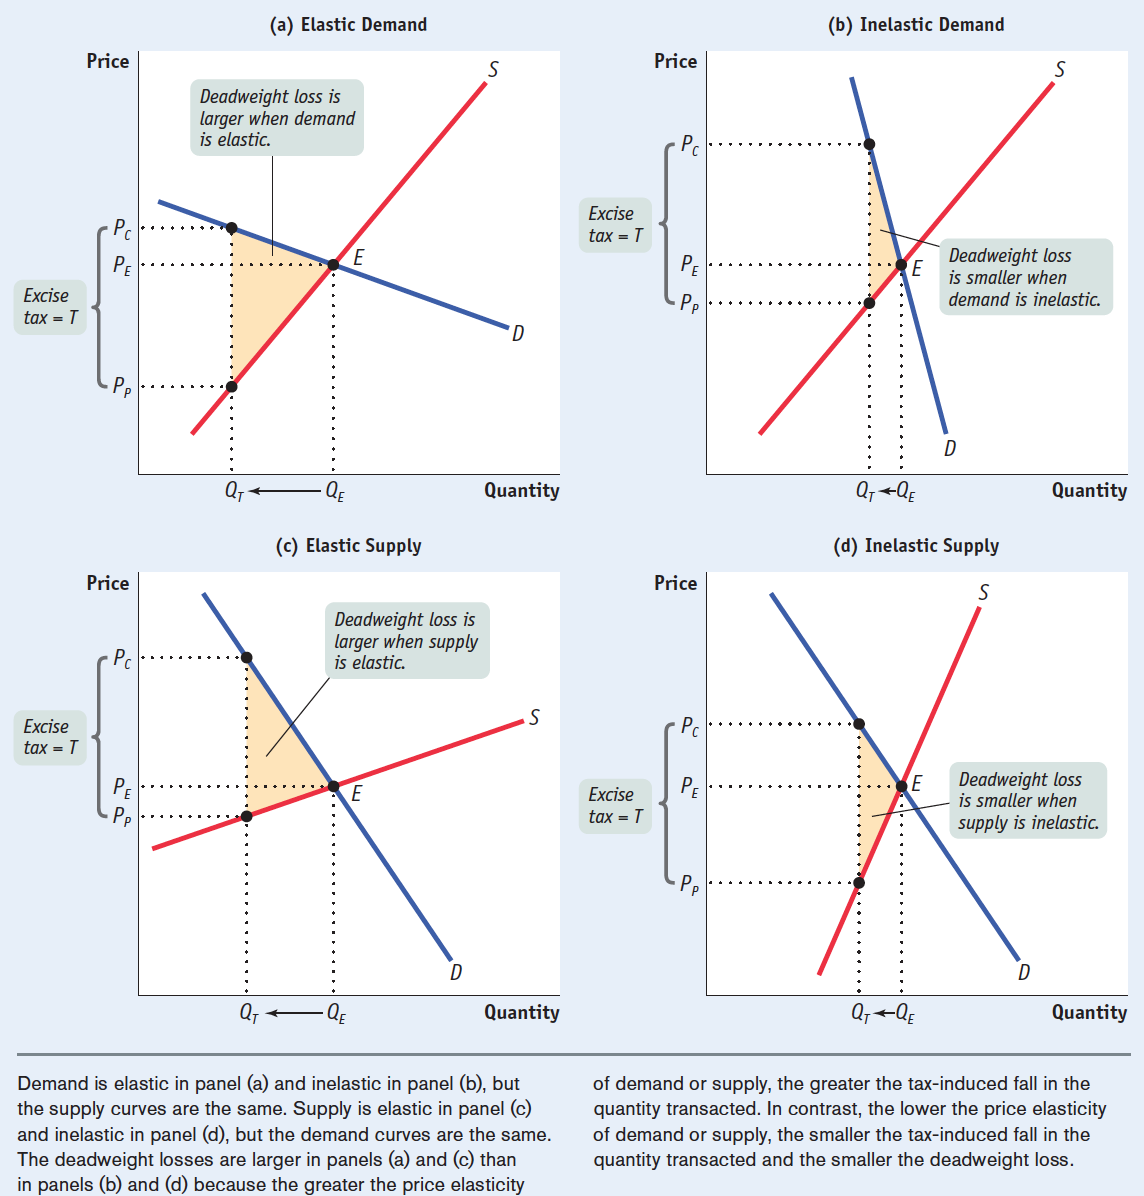
\includegraphics[scale=0.5]{tax5}


%van der berg guido

%production function - tp, mg, fixed feb1
% until returns to scale feb5
% long-run avg total until perfect comp (nec conditions) feb7
% until profitability and market price feb8
% cost of production and efficiency in long-run equilibrium feb12
% monopoly profit-maximising output feb14
% unregulated and regulated feb15
% legal framework feb19
% monopolistic competition feb21
% externalities and public good - social optimal quantity pollution feb 22

\newpage 
\nocite{*}
\printbibliography

\end{document}
